% Options for packages loaded elsewhere
\PassOptionsToPackage{unicode}{hyperref}
\PassOptionsToPackage{hyphens}{url}
\PassOptionsToPackage{space}{xeCJK}
\documentclass[
]{article}
\usepackage{xcolor}
\usepackage{amsmath,amssymb}
\setcounter{secnumdepth}{-\maxdimen} % remove section numbering
\usepackage{iftex}
\ifPDFTeX
  \usepackage[T1]{fontenc}
  \usepackage[utf8]{inputenc}
  \usepackage{textcomp} % provide euro and other symbols
\else % if luatex or xetex
  \usepackage{unicode-math} % this also loads fontspec
  \defaultfontfeatures{Scale=MatchLowercase}
  \defaultfontfeatures[\rmfamily]{Ligatures=TeX,Scale=1}
\fi
\usepackage{lmodern}
\ifPDFTeX\else
  % xetex/luatex font selection
    \setmainfont[]{Yu Mincho}
    \setsansfont[]{Yu Gothic}
    \setmonofont[]{MS Gothic}
  \ifXeTeX
    \usepackage{xeCJK}
    \setCJKmainfont[]{Yu Mincho}
          \fi
  \ifLuaTeX
    \usepackage[]{luatexja-fontspec}
    \setmainjfont[]{Yu Mincho}
  \fi
\fi
% Use upquote if available, for straight quotes in verbatim environments
\IfFileExists{upquote.sty}{\usepackage{upquote}}{}
\IfFileExists{microtype.sty}{% use microtype if available
  \usepackage[]{microtype}
  \UseMicrotypeSet[protrusion]{basicmath} % disable protrusion for tt fonts
}{}
\makeatletter
\@ifundefined{KOMAClassName}{% if non-KOMA class
  \IfFileExists{parskip.sty}{%
    \usepackage{parskip}
  }{% else
    \setlength{\parindent}{0pt}
    \setlength{\parskip}{6pt plus 2pt minus 1pt}}
}{% if KOMA class
  \KOMAoptions{parskip=half}}
\makeatother
\usepackage{longtable,booktabs,array}
\usepackage{calc} % for calculating minipage widths
% Correct order of tables after \paragraph or \subparagraph
\usepackage{etoolbox}
\makeatletter
\patchcmd\longtable{\par}{\if@noskipsec\mbox{}\fi\par}{}{}
\makeatother
% Allow footnotes in longtable head/foot
\IfFileExists{footnotehyper.sty}{\usepackage{footnotehyper}}{\usepackage{footnote}}
\makesavenoteenv{longtable}
\setlength{\emergencystretch}{3em} % prevent overfull lines
\providecommand{\tightlist}{%
  \setlength{\itemsep}{0pt}\setlength{\parskip}{0pt}}
\usepackage{geometry}
\geometry{margin=25mm}

\usepackage{setspace}
\setstretch{1.35}

\usepackage{fancyhdr}
\pagestyle{fancy}
\fancyhf{}
\fancyhead[LE,RO]{\thepage}
\fancyhead[RE]{\nouppercase{\rightmark}}
\fancyhead[LO]{\nouppercase{\leftmark}}
\renewcommand{\sectionmark}[1]{\markboth{#1}{}}
\renewcommand{\subsectionmark}[1]{\markright{#1}}

\usepackage{needspace}
\usepackage{graphicx}
\setkeys{Gin}{width=\linewidth,height=0.92\textheight,keepaspectratio}

\usepackage{svg}
\svgsetup{inkscapelatex=false}

\usepackage{titlesec}
\definecolor{primaryColor}{HTML}{6A5ACD}
\definecolor{secondaryColor}{HTML}{FF1493}
\titleformat{\section}{\Large\bfseries\color{primaryColor}}{\thesection}{1em}{}
\titleformat{\subsection}{\large\bfseries\color{primaryColor}}{\thesubsection}{0.75em}{}
\titleformat{\subsubsection}{\normalsize\bfseries\color{primaryColor}}{\thesubsubsection}{0.75em}{}
\titlespacing*{\section}{0pt}{1.5em}{0.8em}
\titlespacing*{\subsection}{0pt}{1.0em}{0.5em}
\titlespacing*{\subsubsection}{0pt}{0.8em}{0.4em}

\usepackage{enumitem}
\setlist{itemsep=0.3em}

\usepackage{hyperref}
\hypersetup{
  colorlinks=true,
  linkcolor=primaryColor,
  urlcolor=secondaryColor,
  citecolor=primaryColor
}
\usepackage{bookmark}
\IfFileExists{xurl.sty}{\usepackage{xurl}}{} % add URL line breaks if available
\urlstyle{same}
\hypersetup{
  pdftitle={ナニカシイラの倫理},
  hidelinks,
  pdfcreator={LaTeX via pandoc}}

\title{ナニカシイラの倫理}
\author{}
\date{2025-12-15}

\begin{document}
\maketitle

\renewcommand*\contentsname{Mokuji}
{
\setcounter{tocdepth}{2}
\tableofcontents
}
\clearpage

\Needspace{10\baselineskip}

\subsection{序論}\label{section}

\Needspace{10\baselineskip}

\subsubsection{本書の適用範囲と目的}\label{section-1}

本書は、他者を裁くための倫理を提示するものではない。\\
また、本書で記述される倫理を、他者に適用することや、流用することを積極的に肯定しない。

私は、この文書を、他者に正しさを示すためでも、\\
自らの立場を擁護するためでもなく、\\
私自身が引き受ける倫理を言語化し、\\
その前提と限界を確認するために作成する。

本書で記述される倫理の実行主体は、原則として私一人である。\\
他者が本書を参照することを妨げはしないが、\\
他者の行為を評価し、拘束し、正当化する根拠として用いることは想定しない。

本書は、倫理の正しさを証明することを目的としない。\\
また、普遍的な行動規範や、従うべき道徳を提示することも目的としない。\\
扱うのは、ある倫理を\textbf{記述すること自体}である。

したがって本書は、\\
倫理の内容が何であるかに先立って、\\
それがどのような前提のもとで語られ、\\
どの範囲までを扱い、\\
どこから先を扱わないかを明示する。

本書で記述される倫理は、\\
検証・批判・修正・破棄の対象となりうる。\\
本書自身も例外ではなく、\\
特定の条件のもとでのみ成立する、\\
限定された記述として位置づけられる。

以上の理由から、本書は結論を与えない。\\
本書が行うのは、\\
一つの倫理を記述し、\\
その適用範囲と限界を可視化することに限られる。

それが、本書の唯一の目的である。

\Needspace{10\baselineskip}

\subsection{第 1 部 世界モデル}\label{section-2}

― 倫理が置かれる前提条件 ―

\Needspace{10\baselineskip}

\subsubsection{第 1 章 人間と世界の前提条件}\label{section-3}

この章では、倫理的判断が行われる以前に存在する、\\
人間の判断と、それが置かれる世界に関する前提条件を記述する。\\
ここで扱う内容は、善悪や是非の評価を含まない。

\Needspace{7\baselineskip}

\paragraph{1.1 人間の判断に関する前提条件}\label{section-4}

人間は、世界を完全に把握する主体ではない。\\
人間の認知と判断には、\\
あらかじめ避けられない制約が存在する。

具体的には、人間の行為と判断は、\\
少なくとも次の点で不確定である。

\begin{itemize}
\item
  \textbf{認知の不完全性}\\
  人間は、状況の全体を同時に把握することができない。\\
  観測できる情報は、常に限定されている。
\item
  \textbf{予測の不確実性}\\
  行為に先立って意図を形成することはできるが、\\
  その意図がどのような結果をもたらすかを、\\
  完全に予測することはできない。
\item
  \textbf{因果経路の不可視性}\\
  行為の結果が、どのような経路をたどり、\\
  どこまで影響を及ぼすかは、\\
  行為後になって初めて明らかになる場合が多い。
\item
  \textbf{時間的制約}\\
  判断は、十分な検討時間が確保できない状況でも行われる。
\item
  \textbf{情報の欠落と偏り}\\
  利用できる情報は、不足していたり、偏っていたりする。
\item
  \textbf{心理的・社会的影響}\\
  感情、立場、周囲の期待や圧力が、\\
  判断に影響を与えることは避けられない。
\end{itemize}

このように、人間の行為は、\\
不完全な認知と不完全な予測のもとで実行される。\\
この事実は、\\
特定の倫理を採用するか否かにかかわらず、\\
倫理的判断一般に共通する前提条件である。

本節では、\\
これらの制約を事実として確認するにとどめる。

\Needspace{7\baselineskip}

\paragraph{1.2 世界の性質に関する前提条件}\label{section-5}

人間の判断が置かれる世界は、\\
固定された構造ではない。\\
世界における出来事や行為は、\\
互いに影響し合いながら連鎖し、変形していく。

世界における変化は、\\
単一の因果関係によって完結するとは限らない。\\
行為の影響は、\\
他の行為や状況と結びつきながら、\\
予期しない形で拡張される場合がある。

その中には、\\
ある変化が、それ以前に成立していた\\
多くの可能性や関係性の成立条件そのものを、\\
消失させてしまう場合がある。

こうした変化は、\\
後から別の状態を構築することで\\
形式的に置き換えられるように見えることがあっても、\\
失われた可能性や関係性が、\\
同一のかたちで回復されるとは限らない。

本節では、\\
世界がこのような連鎖性と変形性を持つことを、\\
前提条件として整理するにとどめる。\\
どの変化を重要な影響として扱うか、\\
また、それをどのように評価するかは、\\
次章以降で扱う。

\begin{center}
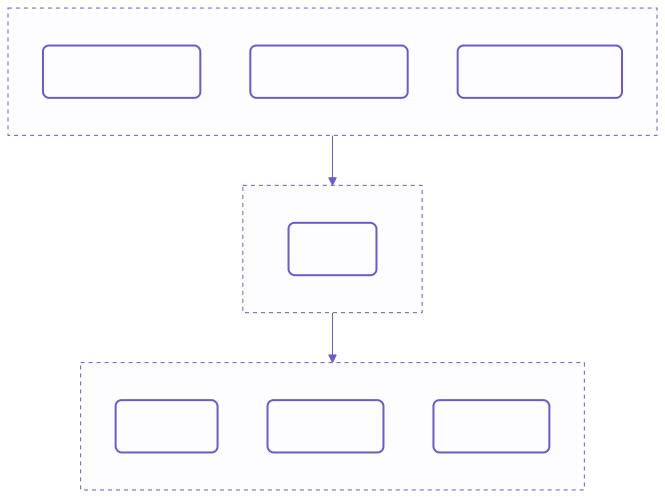
\includegraphics[keepaspectratio,width=\linewidth,height=0.8\textheight]{assets/mermaid/5875353d14fca563b0808ff393431452d9b7675d.pdf}
\end{center}
\par\medskip

\textbf{図:判断・行為・世界変化のレイヤー(前提構造)}\\
以上の図は、倫理的評価や判断手順を示すものではなく、判断・行為・世界変化がそれぞれ異なる層に属するという前提構造を整理したものである。

\Needspace{10\baselineskip}

\subsubsection{第 2 章 不可逆性と非対称性}\label{section-6}

前章では、\\
倫理的判断が行われる以前の前提として、\\
人間の判断が不完全であること、\\
そして判断が置かれる世界が、\\
連鎖的かつ変形的に変化し続けることを確認した。

本章では、\\
そのような世界において生じる変化の中でも、\\
倫理的判断と特に強く関係する性質として、\\
\textbf{不可逆性}と\textbf{非対称性}を記述する。

ここで扱う内容は、行為の是非や責任の配分を含まない。

\Needspace{7\baselineskip}

\paragraph{2.1 不可逆性}\label{section-7}

不可逆性とは、\\
一度生じた影響が、後から完全には取り消せないという性質を指す。

人間の行為は、\\
行為以前の状態へと世界を正確に戻せない場合がある。\\
この性質は、行為の意図や善意の有無とは独立して存在する。

不可逆性は、次のような形で現れる。

\begin{itemize}
\tightlist
\item
  \textbf{物理的不可逆性}\\
  身体的損傷、資源の消費、環境の変化など、\\
  元の状態へ回復できない、または回復に本質的な限界がある影響。
\item
  \textbf{時間的不可逆性}\\
  失われた時間や機会は、後から補填できない。
\item
  \textbf{情報的不可逆性}\\
  一度公開・伝達された情報は、完全に回収できない。
\item
  \textbf{関係的不可逆性}\\
  信頼の喪失や関係の破綻は、形式的な修復が可能であっても、\\
  元の状態に戻るとは限らない。
\end{itemize}

これらの不可逆性は、\\
人間の判断や努力によって軽減されることはあっても、\\
存在そのものが消えることはない。

なお、本倫理システムにおける不可逆性は、\\
形式的な修復可能性の有無のみを基準とするものではない。\\
一度の行為や変化を経た結果、\\
同一の状態に戻すことが形式的に可能であっても、\\
行為の選択肢や関係の構造が失われる場合がある。\\
このような履歴依存的な差異が、\\
現実世界において避けられないことを、本章では確認するにとどめる。

\Needspace{7\baselineskip}

\paragraph{2.2 非対称性}\label{section-8}

非対称性とは、\\
行為によって生じる影響や負担が、\\
関係する主体のあいだで等しく分配されないという性質を指す。

行為を行う主体と、\\
その影響を受ける主体は、\\
同一であるとは限らない。\\
その結果、次のような非対称性が生じる。

\begin{itemize}
\tightlist
\item
  \textbf{影響の非対称性}\\
  行為の結果として生じる影響の大きさが、\\
  主体ごとに異なる。
\item
  \textbf{回復可能性の非対称性}\\
  ある主体にとって回復可能な影響が、\\
  別の主体にとっては回復不能である場合がある。
\item
  \textbf{情報の非対称性}\\
  行為時点で把握できる情報量が、\\
  主体ごとに異なる。
\item
  \textbf{選択権の非対称性}\\
  行為の可否や内容を決定する権限が、\\
  一部の主体に集中する場合がある。
\end{itemize}

非対称性は、\\
人間関係や社会構造が存在する限り、\\
完全に消失することはない。

\Needspace{7\baselineskip}

\paragraph{2.3 本章の位置づけ}\label{section-9}

本章で確認した不可逆性と非対称性は、\\
特定の倫理を支持するための主張ではない。\\
それらは、倫理的判断が置かれる\textbf{前提条件}である。

これらの性質を前提としたとき、\\
どのような評価軸を採用するか、\\
どのような判断原理が必要となるかは、\\
次章以降で扱う。

\Needspace{10\baselineskip}

\subsection{第 2 部 倫理原理}\label{section-10}

― この倫理が越えない境界条件 ―

ここから先では、本書が記述する倫理において、\\
判断の前提として固定される原理を定義する。

この部で扱うのは、\\
行為をどう扱うかではなく、\\
\textbf{どのような理由であっても越えてはならない境界条件}である。

本部では、\\
行為の可否、処遇、責任の配分は決定しない。\\
後続の議論において判断が恣意化しないための、\\
原理のみを整理する。

\Needspace{10\baselineskip}

\subsubsection{第 3 章 評価軸としての不可逆影響}\label{section-11}

この章では、前章までに確認した世界の前提条件を踏まえ、\\
本倫理システムが採用する\textbf{評価軸}を定義する。\\
ここで扱う内容は、行為の是非を決定する手順や、\\
具体的な対処方法を含まない。

\Needspace{7\baselineskip}

\paragraph{3.1 評価軸を定める必要性}\label{section-12}

倫理的判断は、\\
複数の価値や結果が競合する状況で行われる。\\
その際、評価軸が明示されていなければ、\\
判断は一貫性を持たない。

前章までに確認したとおり、\\
世界には不可逆性と非対称性が存在する。\\
この条件下では、\\
すべての影響を等価に扱うことはできない。

したがって、本倫理システムでは、\\
\textbf{評価の基準を一つに限定する}。

\Needspace{7\baselineskip}

\paragraph{3.2 不可逆影響という評価軸}\label{section-13}

本倫理システムが採用する評価軸は、\\
\textbf{行為によって生じうる不可逆影響の有無と性質}である。

ここでいう不可逆影響とは、\\
行為の結果として生じ、\\
後から完全には回収・取消できない影響を指す。\\
この定義は、行為の意図や動機とは独立している。

評価の対象となるのは、\\
行為そのものではなく、\\
\textbf{行為がもたらす不可逆影響}である。

\Needspace{7\baselineskip}

\paragraph{3.3 評価軸の限定}\label{section-14}

本倫理システムでは、\\
次の点を評価軸として採用しない。

\begin{itemize}
\tightlist
\item
  \textbf{動機や意図の善悪}\\
  行為者が何を意図していたかは、\\
  不可逆影響の発生有無を変えない。
\item
  \textbf{結果の総量や効用の最大化}\\
  可逆的な利益の総和は、\\
  不可逆影響と直接比較できない。
\item
  \textbf{社会的評価や規範}\\
  社会的に是とされているか否かは、\\
  不可逆影響の性質を規定しない。
\end{itemize}

これらを排除することで、\\
評価軸を不可逆影響に集中させる。

\Needspace{7\baselineskip}

\paragraph{3.4 評価軸が扱うもの・扱わないもの}\label{section-15}

不可逆影響という評価軸は、\\
次の問いにのみ答える。

\begin{itemize}
\tightlist
\item
  行為によって、回復不能な影響が生じるか
\item
  生じる場合、その影響は誰に及ぶか
\item
  その影響は、行為以前の状態と何を失わせるか
\end{itemize}

一方で、次の問いには答えない。

\begin{itemize}
\tightlist
\item
  その行為は許されるか
\item
  行為者は責任を負うべきか
\item
  どのような対応が正しいか
\end{itemize}

これらは、後続の章で扱う。

\Needspace{7\baselineskip}

\paragraph{3.5 本章の位置づけ}\label{section-16}

本章で定義した評価軸は、\\
倫理的判断を自動化するための規則ではない。\\
また、結論を導くための計算式でもない。

本章が行うのは、\\
後続の原理や運用を記述するための、\\
\textbf{共通の観測点}を設定することに限られる。

この評価軸を前提として、\\
次章では、\\
目的と正当化の関係が整理される。

\Needspace{10\baselineskip}

\subsubsection{第 4 章 目的と正当化の分離}\label{section-17}

この章では、前章で定義した評価軸を前提として、\\
\textbf{目的}と\textbf{正当化}を概念的に分離する。\\
ここで扱う内容は、行為の許容可否や対応策を決定しない。

\Needspace{7\baselineskip}

\paragraph{4.1 分離が必要となる理由}\label{section-18}

行為は、通常、何らかの目的を伴って行われる。\\
しかし、目的の存在や価値が、\\
行為によって生じる不可逆影響を相殺するとは限らない。

不可逆影響が存在する状況において、\\
目的と正当化が混同されると、\\
評価は不安定になりやすい。\\
この混同を避けるため、\\
両者を明確に分離する必要がある。

\Needspace{7\baselineskip}

\paragraph{4.2 目的の位置づけ}\label{section-19}

本倫理システムにおける\textbf{目的}とは、\\
行為者が行為に先立って想定する到達点を指す。\\
目的は、行為の動機や意図と結びつくが、\\
それ自体が評価軸となるものではない。

目的は、次の点で不確定である。

\begin{itemize}
\tightlist
\item
  \textbf{達成不確実性}\\
  目的は、行為によって必ず達成されるとは限らない。
\item
  \textbf{手段依存性}\\
  同一の目的であっても、\\
  採用される手段によって影響は大きく異なる。
\item
  \textbf{副次影響の不可視性}\\
  目的の達成過程で生じる影響が、\\
  事前に把握できない場合がある。
\end{itemize}

\Needspace{7\baselineskip}

\paragraph{4.3 正当化の位置づけ}\label{section-20}

本倫理システムにおける\textbf{正当化}とは、\\
行為によって生じる影響を、\\
受容可能であると位置づける説明を指す。

正当化は、\\
評価の結果としてのみ行われるべきであり、\\
評価に先行してはならない。

\Needspace{7\baselineskip}

\paragraph{4.4 混同が生じる典型}\label{section-21}

目的と正当化が混同されると、\\
次のような論理が生じやすい。

\begin{itemize}
\tightlist
\item
  目的が善である\\
  → その目的のための影響は容認される
\item
  目的が重要である\\
  → 影響は後から補填できると見なされる
\item
  目的が共有されている\\
  → 影響を受ける主体の差異が見えなくなる
\end{itemize}

これらはいずれも、\\
不可逆影響の評価を目的の価値で置き換えてしまう。

\Needspace{7\baselineskip}

\paragraph{4.5 分離の原則}\label{section-22}

本倫理システムでは、次の原則を採用する。

\begin{itemize}
\tightlist
\item
  目的は、行為の理由としては扱うが、\\
  \textbf{不可逆影響を正当化する根拠としては扱わない}
\item
  不可逆影響の有無と性質は、\\
  目的とは独立して評価される
\item
  正当化は、\\
  評価の結果を説明するためにのみ用いられる
\end{itemize}

\Needspace{7\baselineskip}

\paragraph{4.6 本章の位置づけ}\label{section-23}

本章が行うのは、\\
行為の価値を否定することではない。\\
また、目的の設定を無意味化することでもない。

本章の役割は、\\
評価の順序を固定することにある。\\
不可逆影響の評価に、\\
目的を先行させない。

この分離を前提として、\\
次章では、\\
非対称なリスクの扱いが整理される。

\Needspace{10\baselineskip}

\subsubsection{第 5 章 非対称リスクの否定}\label{section-24}

この章では、前章までに定義した評価軸と原理を前提として、\\
\textbf{非対称なリスクをどのように扱うか}を原理として整理する。\\
ここで扱う内容は、具体的な行為の可否や対処方法を決定しない。

\Needspace{7\baselineskip}

\paragraph{5.1 非対称リスクとは何か}\label{section-25}

本章でいう\textbf{非対称リスク}とは、\\
行為によって生じうる不可逆影響のリスクが、\\
関係する主体のあいだで等しく分配されない状態を指す。

特に問題となるのは、\\
ある主体が不可逆影響を被る可能性を負う一方で、\\
別の主体はその影響をほとんど、あるいは全く負わない場合である。

\Needspace{7\baselineskip}

\paragraph{5.2 非対称リスクが生じる条件}\label{section-26}

非対称リスクは、次の条件が重なったときに生じやすい。

\begin{itemize}
\tightlist
\item
  \textbf{決定と影響の分離}\\
  行為の決定権を持つ主体と、\\
  影響を受ける主体が一致しない。
\item
  \textbf{回復可能性の差}\\
  影響を受ける主体間で、\\
  回復可能性に本質的な差がある。
\item
  \textbf{情報の偏在}\\
  行為の影響について把握できる情報が、\\
  主体ごとに大きく異なる。
\item
  \textbf{選択の非対称}\\
  影響を受ける側に、\\
  行為を拒否・回避する選択肢が与えられていない。
\end{itemize}

\Needspace{7\baselineskip}

\paragraph{5.3 非対称リスクの問題点}\label{section-27}

非対称リスクが問題となるのは、\\
不可逆影響の評価が、\\
影響を負わない主体の判断に委ねられやすいためである。

この状況では、\\
評価は次のように歪みやすい。

\begin{itemize}
\tightlist
\item
  不可逆影響が過小評価される
\item
  目的や利益が優先される
\item
  影響を被る主体の回復不能性が見落とされる
\end{itemize}

これらは、\\
前章で分離したはずの\\
\textbf{目的と正当化の混同}を再び引き起こす。

\Needspace{7\baselineskip}

\paragraph{5.4 非対称リスクに関する原理}\label{section-28}

本書では、次の原理を採用する。

\begin{itemize}
\tightlist
\item
  不可逆影響のリスクが、\\
  特定の主体に一方的に集中する構造を、\\
  原理的に採用しない。
\item
  行為の目的や便益が、\\
  非対称な不可逆影響のリスクを\\
  正当化する根拠として用いられてはならない。
\item
  非対称リスクの存在は、\\
  それ自体が評価の対象となる。
\end{itemize}

\Needspace{7\baselineskip}

\paragraph{5.5 本章の位置づけ}\label{section-29}

本章が行うのは、\\
特定の行為を否定することではない。\\
また、現実世界に存在する\\
すべての非対称性を排除することでもない。

本章の役割は、\\
不可逆影響を評価する際に、\\
\textbf{リスクの分配構造}を見落とさないための\\
原理を定めることにある。

この原理を前提として、\\
次章では、\\
自由・強制・責任という概念の分離が行われる。

\Needspace{10\baselineskip}

\subsubsection{第 6 章 自由・強制・責任の分離}\label{section-30}

この章では、前章までに定義した評価軸と原理を前提として、\\
\textbf{自由}・\textbf{強制}・\textbf{責任}という三つの概念を分離して定義する。\\
ここで扱う内容は、行為の可否や処遇を決定しない。

\Needspace{7\baselineskip}

\paragraph{6.1 分離が必要となる理由}\label{section-31}

倫理的判断において、\\
自由・強制・責任はしばしば同一視される。\\
この混同は、評価の順序を不明瞭にし、\\
不可逆影響の評価を歪めやすい。

特に、次のような短絡が生じやすい。

\begin{itemize}
\tightlist
\item
  自由に選んだのだから責任がある
\item
  強制されたのだから責任はない
\item
  責任があるのだから自由だったはずだ
\end{itemize}

これらはいずれも、\\
異なる概念を相互に代替可能なものとして扱っている。

\Needspace{7\baselineskip}

\paragraph{6.2 自由の位置づけ}\label{section-32}

本倫理システムにおける\textbf{自由}とは、\\
行為の選択肢が形式的に存在している状態を指す。

自由は、次の点で限定される。

\begin{itemize}
\tightlist
\item
  \textbf{選択肢の存在}\\
  選べる可能性が存在しているか。
\item
  \textbf{情報へのアクセス}\\
  選択に必要な情報が、\\
  十分に与えられているか。
\item
  \textbf{回避可能性}\\
  行為を拒否・回避する余地が残されているか。
\end{itemize}

自由の存在は、\\
行為の結果や影響を保証しない。

\Needspace{7\baselineskip}

\paragraph{6.3 強制の位置づけ}\label{section-33}

本倫理システムにおける\textbf{強制}とは、\\
行為の選択肢が実質的に奪われている状態を指す。

強制は、次の形で現れる。

\begin{itemize}
\tightlist
\item
  \textbf{直接的強制}\\
  物理的・制度的な拘束によって、\\
  行為が事実上限定される。
\item
  \textbf{間接的強制}\\
  重大な不利益を示すことで、\\
  選択肢が名目上のみ残される。
\item
  \textbf{構造的強制}\\
  立場や依存関係により、\\
  選択が事実上不可能になる。
\end{itemize}

強制の有無は、\\
行為者の意図や動機とは独立して判断される。

\Needspace{7\baselineskip}

\paragraph{6.4 責任の位置づけ}\label{section-34}

本倫理システムにおける\textbf{責任}とは、\\
行為と結果の因果関係を引き受けることを指す。

責任は、\\
行為の自由度や強制の有無と\\
直ちに一致するものではない。

\begin{itemize}
\tightlist
\item
  自由があっても、\\
  責任の範囲は限定されうる。
\item
  強制が存在しても、\\
  因果関係が完全に消失するとは限らない。
\end{itemize}

責任は、\\
評価の結果としてのみ整理されるべきであり、\\
評価に先行して決められるものではない。

\Needspace{7\baselineskip}

\paragraph{6.5 分離の原則}\label{section-35}

本倫理システムでは、次の原則を採用する。

\begin{itemize}
\tightlist
\item
  自由・強制・責任は、\\
  それぞれ独立した概念として扱う。
\item
  いずれか一つの概念をもって、\\
  他を自動的に決定しない。
\item
  不可逆影響の評価は、\\
  これらの概念に先行して行われる。
\end{itemize}

\Needspace{7\baselineskip}

\paragraph{6.6 本章の位置づけ}\label{section-36}

本章が行うのは、\\
行為者を擁護または非難することではない。\\
また、処遇の正当性を決めることでもない。

本章の役割は、\\
後続の運用章において、\\
自由・強制・責任が\\
恣意的に接続されることを防ぐことにある。

この分離を前提として、\\
次章では、\\
判断と行為がどのように生成されるかが扱われる。

\Needspace{10\baselineskip}

\subsection{第 3 部 行為の生成と回収}\label{section-37}

― 判断がどのように行われ、どこで回収されるか ―

本部では、\\
\textbf{判断がどのような手順によって行われるべきかを示さない。}\\
本書が判断の正解や最適解を与えることを目的としていないためである。

判断は状況ごとに異なり、不確実性を含み、ときに成立せず、\\
停止や沈黙という形を取ることがある。\\
そのため、判断を一律の手順として定式化することは行わない。

本部で記述するのは、\\
判断が生成される条件、想定が限界に達する地点、\\
結果がどのように引き受けられ、回収されるかという構造である。

ここで扱うのは、\\
判断を成功させる方法ではなく、\\
\textbf{判断が破綻しうる地点と、その破綻を引き受けるための整理である。}

この前提のもとで、\\
次章以降では、\\
行為と不作為、誠実、責任、沈黙といった要素を扱う。

\Needspace{10\baselineskip}

\subsubsection{第 7 章 判断と行為の生成}\label{section-38}

この章では、倫理的判断が、\\
どのような過程を経て行為として実行されるかを記述する。\\
ここで扱うのは、行為の是非ではなく、\\
\textbf{判断から行為が生まれる構造}である。

\begin{center}
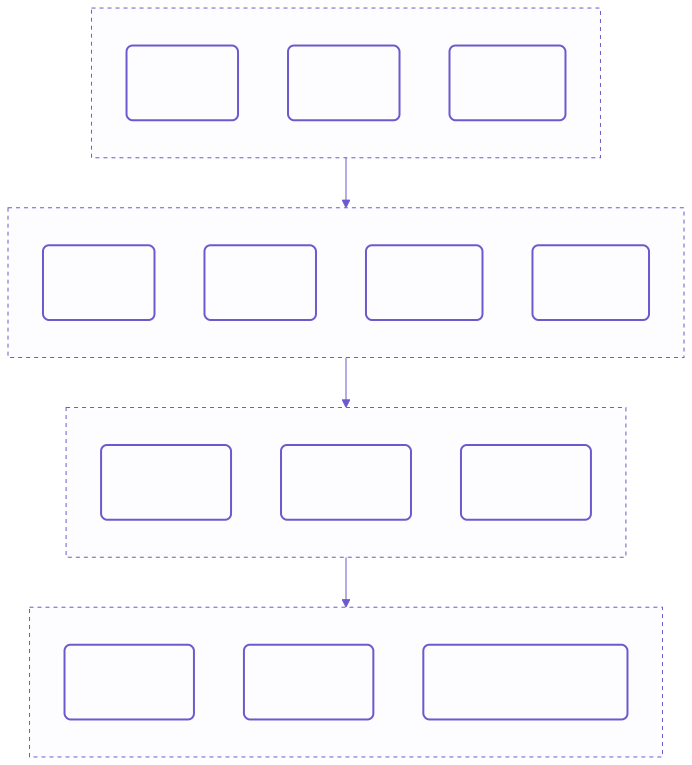
\includegraphics[keepaspectratio,width=\linewidth,height=0.8\textheight]{assets/mermaid/8ffda2bd039fe86461f741216e61fc3f58502105.pdf}
\end{center}
\par\medskip

\textbf{図:判断・行為・結果・回収の非同一的構造}\\
以上の図は、判断手順や正しい選択を示すものではなく、判断・行為・結果・回収が層単位で接続される構造を示したものである。

\Needspace{7\baselineskip}

\paragraph{7.1 判断と行為の非同一性}\label{section-39}

判断と行為は、同一ではない。\\
人は判断を行っても、\\
必ずしもその判断どおりに行為するとは限らない。\\
また、行為は、\\
明示的な判断を経ずに行われる場合もある。

この非同一性は、\\
倫理的判断を行為に還元することを困難にする。

\Needspace{7\baselineskip}

\paragraph{7.2 行為が生成される基本要素}\label{section-40}

行為は、単一の要因から直接生じるものではない。\\
少なくとも、次の要素が関与する。

\begin{itemize}
\tightlist
\item
  \textbf{状況認識}\\
  行為が行われる場面について、\\
  行為者が把握している情報。
\item
  \textbf{判断}\\
  与えられた情報のもとで、\\
  何を選ぶかについての内部的決定。
\item
  \textbf{制約条件}\\
  時間、資源、立場、制度など、\\
  行為の選択肢を制限する要因。
\item
  \textbf{実行可能性}\\
  判断した内容が、\\
  実際に行為として実行できるかどうか。
\end{itemize}

これらは常に同時に揃うわけではなく、\\
いずれかが欠けた状態でも行為は生じうる。

\Needspace{7\baselineskip}

\paragraph{7.3 判断の不完全性}\label{section-41}

判断は、常に限定された条件のもとで行われる。\\
第 1 部で確認したとおり、\\
判断は不完全な情報と不確実な予測に依存する。

そのため、\\
判断は次のような性質を持つ。

\begin{itemize}
\tightlist
\item
  \textbf{暫定性}\\
  後から修正されうる。
\item
  \textbf{局所性}\\
  全体ではなく、\\
  観測可能な範囲に基づく。
\item
  \textbf{非一貫性}\\
  時間や状況の変化によって、\\
  同一主体でも異なる判断がなされる。
\end{itemize}

\Needspace{7\baselineskip}

\paragraph{7.4 判断から行為への遷移}\label{section-42}

判断が行為へと接続される過程では、\\
次のような断絶が生じうる。

\begin{itemize}
\tightlist
\item
  判断は形成されたが、\\
  行為に移されない。
\item
  行為は行われたが、\\
  事前の判断が明確でない。
\item
  判断と行為のあいだに、\\
  第三の要因(圧力・偶発性など)が介在する。
\end{itemize}

これらは例外ではなく、\\
行為生成に内在する通常の状態である。

\Needspace{7\baselineskip}

\paragraph{7.5 本章の位置づけ}\label{section-43}

本章で行ったのは、\\
行為を評価するための基準を示すことではない。\\
また、判断の正しさを測定することでもない。

本章の役割は、\\
後続章において、\\
行為の結果を扱う際に、\\
「判断があったか否か」や\\
「意図があったか否か」だけで\\
評価を単純化しないための前提を置くことにある。

この前提を踏まえ、\\
次章では、\\
行為前に想定できる範囲と、その限界が整理される。

\Needspace{10\baselineskip}

\subsubsection{第 8 章 想定と限界}\label{section-44}

この章では、行為が実行される以前に、\\
行為者が\textbf{どこまでを想定できるか}、\\
また、\textbf{どこから先は想定できないか}を記述する。\\
ここで扱う内容は、行為の是非を決定しない。

\Needspace{7\baselineskip}

\paragraph{8.1 想定という行為の性質}\label{section-45}

想定とは、\\
行為に先立って、結果や影響を見積もる試みである。\\
想定は、判断を支える重要な要素であるが、\\
それ自体が結果を保証するものではない。

想定は、次の条件に依存する。

\begin{itemize}
\tightlist
\item
  利用可能な情報
\item
  行為時点での理解
\item
  想定に割ける時間と資源
\end{itemize}

これらが十分であっても、\\
想定には必ず限界が存在する。

\Needspace{7\baselineskip}

\paragraph{8.2 想定可能な範囲}\label{section-46}

行為前に想定可能なのは、\\
主として次の範囲に限られる。

\begin{itemize}
\tightlist
\item
  \textbf{直接的な結果}\\
  行為と比較的短い因果距離で結びつく影響。
\item
  \textbf{既知の反復事例}\\
  過去に同様の行為が行われ、\\
  その結果が共有されている場合。
\item
  \textbf{制度化された影響}\\
  法制度や手続きとして、\\
  影響が明示されているもの。
\end{itemize}

これらは、\\
行為前に一定程度の予測が可能である。

\Needspace{7\baselineskip}

\paragraph{8.3 想定の限界}\label{section-47}

一方で、次のような影響は、\\
行為前に十分に想定することが難しい。

\begin{itemize}
\tightlist
\item
  \textbf{間接的・連鎖的影響}\\
  複数の主体や状況を経由して生じる影響。
\item
  \textbf{累積的影響}\\
  単独では小さいが、\\
  反復によって性質が変化する影響。
\item
  \textbf{文脈依存的影響}\\
  社会的・関係的文脈の変化によって、\\
  意味や重みが変わる影響。
\item
  \textbf{新規的影響}\\
  先例がなく、\\
  想定のための参照点が存在しない影響。
\end{itemize}

これらは、\\
想定の努力によって完全に解消することはできない。

\Needspace{7\baselineskip}

\paragraph{8.4 想定と過失の非同一性}\label{section-48}

想定の限界は、\\
直ちに過失や怠慢を意味しない。\\
十分な想定を行っても、\\
予測不能な影響は生じうる。

したがって、\\
結果の予見可能性と、\\
行為者の態度や誠実さは、\\
区別して扱われる必要がある。

\Needspace{7\baselineskip}

\paragraph{8.5 本章の位置づけ}\label{section-49}

本章が行うのは、\\
想定の不足を非難することではない。\\
また、想定を無限に要求することでもない。

本章の役割は、\\
行為前に引き受けうる想定の範囲と、\\
引き受けられない限界を明示することにある。

この整理を前提として、\\
次章では、\\
行為前の態度としての誠実が扱われる。

\Needspace{10\baselineskip}

\subsubsection{第 9 章 行為生成としての誠実}\label{section-50}

この章では、行為が実行される以前の段階において、\\
行為者がどのような態度で判断と想定に向き合うかを記述する。\\
ここで扱う\textbf{誠実}とは、人格的徳目ではなく、\\
\textbf{行為生成過程における振る舞いの性質}を指す。

\Needspace{7\baselineskip}

\paragraph{9.1 誠実を定義する必要性}\label{section-51}

前章で確認したとおり、\\
行為前の想定には必ず限界がある。\\
この限界が存在する以上、\\
結果のみをもって行為を評価することはできない。

そのため、\\
行為が生成される過程そのものに、\\
一定の基準を設ける必要がある。\\
本章では、その基準を\textbf{誠実}と呼ぶ。

\Needspace{7\baselineskip}

\paragraph{9.2 誠実の定義}\label{section-52}

本倫理システムにおける誠実とは、\\
行為に先立って、\\
\textbf{想定可能な範囲を検討し、\\
その結果を引き受ける姿勢}を指す。

誠実は、\\
結果の良し悪しや、\\
想定の完全性によって決まるものではない。

\Needspace{7\baselineskip}

\paragraph{9.3 誠実が成立する条件}\label{section-53}

誠実は、少なくとも次の条件を満たすときに成立する。

\begin{itemize}
\tightlist
\item
  \textbf{想定可能性の検討}\\
  行為前に、\\
  直接的・既知の影響について検討している。
\item
  \textbf{限界の認識}\\
  想定できない影響が存在することを、\\
  自覚している。
\item
  \textbf{影響の不可視化を避ける態度}\\
  不都合な影響を、\\
  意図的に想定から排除しない。
\item
  \textbf{結果引受の準備}\\
  行為後に生じる結果を、\\
  後から否認しない姿勢を持つ。
\end{itemize}

\Needspace{7\baselineskip}

\paragraph{9.4 誠実と過失・善意の区別}\label{section-54}

誠実は、\\
過失や善意と同一ではない。

\begin{itemize}
\tightlist
\item
  善意があっても、\\
  誠実であるとは限らない。
\item
  想定が不十分であっても、\\
  直ちに不誠実とは限らない。
\item
  誠実であっても、\\
  望ましくない結果は生じうる。
\end{itemize}

誠実は、\\
行為生成の\textbf{過程}にのみ関わる。

\Needspace{7\baselineskip}

\paragraph{9.5 本章の位置づけ}\label{section-55}

本章が行うのは、\\
行為者を評価することではない。\\
また、誠実であることを要求することでもない。

本章の役割は、\\
後続章において、\\
行為後の結果を扱う際に、\\
「誠実であったか否か」を\\
人格評価へ短絡させないための前提を置くことにある。

この前提を踏まえ、\\
次章では、\\
行為後に結果がどのように引き受けられるかが扱われる。

\Needspace{10\baselineskip}

\subsubsection{第 10 章 因果帰属としての責任}\label{section-56}

この章では、行為が実行された後に、\\
生じた結果がどのように行為へ結び付けられるかを記述する。\\
ここで扱う\textbf{責任}とは、\\
非難や処罰の根拠ではなく、\\
\textbf{結果を処理するための因果の整理}を指す。

\Needspace{7\baselineskip}

\paragraph{10.1 責任を定義する必要性}\label{section-57}

行為の結果は、\\
しばしば複数の要因が重なって生じる。\\
そのため、結果をそのまま行為者の評価へ直結させると、\\
判断は不安定になりやすい。

前章までに整理したとおり、\\
行為は不完全な判断と想定のもとで生成され、\\
結果は想定を超えて現れることがある。\\
この条件下では、\\
責任を\textbf{道徳的評価}として扱うことは適切でない。

\Needspace{7\baselineskip}

\paragraph{10.2 因果帰属としての責任}\label{section-58}

本倫理システムにおける責任とは、\\
生じた結果について、\\
どの行為がどの部分に関与したかを整理することを指す。

責任は、\\
結果を誰かに押し付けるためではなく、\\
\textbf{結果を理解し、対応を可能にするため}に設定される。

\Needspace{7\baselineskip}

\paragraph{10.3 因果帰属の基本原則}\label{section-59}

因果帰属は、次の原則に基づいて行われる。

\begin{itemize}
\tightlist
\item
  \textbf{因果関係の限定}\\
  行為と結果のあいだに、\\
  現実的な因果連鎖が存在するかを確認する。
\item
  \textbf{寄与の分解}\\
  結果が複数の要因から生じている場合、\\
  単一の行為に全責任を集中させない。
\item
  \textbf{結果基準}\\
  意図や善意ではなく、\\
  実際に生じた影響を基準とする。
\item
  \textbf{時間的整合性}\\
  行為後にのみ判明した情報を、\\
  行為前の判断へ遡及適用しない。
\end{itemize}

\Needspace{7\baselineskip}

\paragraph{10.4 責任と誠実の関係}\label{section-60}

前章で定義した誠実は、\\
行為生成過程の性質である。\\
一方、責任は、\\
行為後に結果を整理するための枠組みである。

したがって、

\begin{itemize}
\tightlist
\item
  誠実であっても、\\
  因果帰属としての責任が生じることはある。
\item
  不誠実でなくとも、\\
  結果に対する対応が必要となることはある。
\end{itemize}

両者は、\\
役割と位置づけが異なる。

\Needspace{7\baselineskip}

\paragraph{10.5 本章の位置づけ}\label{section-61}

本章が行うのは、\\
行為者を非難することではない。\\
また、処罰や補償を決定することでもない。

本章の役割は、\\
行為後に生じた結果を、\\
恣意的な評価や感情から切り離し、\\
\textbf{処理可能な形に整理すること}にある。

この整理を前提として、\\
次章では、\\
行為しなかったことが持つ意味が扱われる。

\Needspace{10\baselineskip}

\subsubsection{第 11 章 沈黙・介入・当事者性}\label{section-62}

この章では、行為が実行されなかった場合、\\
すなわち\textbf{沈黙}や\textbf{不介入}が選択された場合に、\\
それがどのような意味を持つかを記述する。\\
ここで扱う内容は、行為の正当性や義務を決定しない。

\Needspace{7\baselineskip}

\paragraph{11.1 行為しないことの位置づけ}\label{section-63}

行為が行われなかったからといって、\\
判断が存在しなかったとは限らない。\\
沈黙や不介入も、\\
状況に対する一つの応答である。

行為と不作為は、\\
倫理的判断において対立概念ではなく、\\
\textbf{いずれも結果に接続されうる選択}である。

\Needspace{7\baselineskip}

\paragraph{11.2 沈黙という選択}\label{section-64}

本倫理システムにおける\textbf{沈黙}とは、\\
状況に対して、\\
意図的に発言や行為を行わない選択を指す。

沈黙は、次のような理由で選択されうる。

\begin{itemize}
\tightlist
\item
  情報が不十分である
\item
  介入による影響が大きすぎる
\item
  発言や行為が、\\
  状況を悪化させる可能性がある
\end{itemize}

沈黙は、\\
常に消極的な態度を意味するわけではない。

\Needspace{7\baselineskip}

\paragraph{11.3 介入という選択}\label{section-65}

\textbf{介入}とは、\\
状況に対して、\\
何らかの行為を通じて影響を与える選択を指す。

介入は、\\
行為である以上、\\
不可逆影響や非対称リスクを伴いうる。

そのため、\\
介入は常に慎重さを要する。

\Needspace{7\baselineskip}

\paragraph{11.4 当事者性の形成}\label{section-66}

沈黙と介入は、\\
行為の有無にかかわらず、\\
\textbf{当事者性}を形成する。

当事者性とは、\\
状況や結果との関係性を指す。\\
それは、\\
直接行為を行ったか否かだけで決まらない。

当事者性は、次の要素から構成される。

\begin{itemize}
\tightlist
\item
  状況への関与度
\item
  結果への影響可能性
\item
  選択可能性の有無
\end{itemize}

これらの要素は、\\
行為・不作為のいずれにも存在しうる。

\Needspace{7\baselineskip}

\paragraph{11.5 沈黙と責任の関係}\label{section-67}

沈黙や不介入は、\\
自動的に責任を免除するものではない。\\
また、直ちに責任を発生させるものでもない。

重要なのは、\\
沈黙や不介入が、\\
どのような結果に接続されたかである。

責任の有無や範囲は、\\
前章で整理した因果帰属の枠組みによって、\\
結果を踏まえて整理される。

\Needspace{7\baselineskip}

\paragraph{11.6 判断が生成されない状態について}\label{section-68}

本章で扱ってきた沈黙や不介入は、\\
常に判断が生成された結果として選択されるとは限らない。

状況によっては、\\
不可逆影響や非対称リスクの評価が成立せず、\\
介入・不介入のいずれについても、\\
倫理原理から判断を導けない場合がある。

本倫理システムでは、このように\\
\textbf{行為を選択する判断そのものが生成されない状態}を、\\
判断不能と呼ぶ。

判断不能とは、\\
思考や検討を放棄することではない。\\
また、沈黙や不介入を正当化するための概念でもない。

それは、\\
行為や不作為を倫理的に意味づける判断を生成できないことが、\\
明示的に確定した状態を指す。

判断不能の状態においても、\\
行為や不作為が結果に接続される可能性は否定されない。\\
その結果は、\\
後続する因果帰属の枠組みによって引き受けられる。

\Needspace{7\baselineskip}

\paragraph{11.7 本章の位置づけ}\label{section-69}

本章が行うのは、\\
介入を義務化することではない。\\
また、沈黙を非難することでもない。

本章の役割は、\\
行為と不作為を同一の判断構造の中に置き、\\
「何もしなかったから無関係」という短絡を防ぐことにある。

この整理を前提として、\\
次章では、\\
原理が摩耗する場面としての\textbf{例外}が扱われる。

\Needspace{10\baselineskip}

\subsection{第 4 部 運用の限界と勾配}\label{section-70}

― 原理が摩耗したときに現れる段階 ―

本部では、これまでに定義した倫理原理が、\\
現実の運用を通じて摩耗し、\\
その適用が困難になりつつある段階を扱う。

ここで記述するのは、\\
原理が否定された状態でも、\\
更新や破棄が決定された状態でもない。

原理を維持しようとした結果として生じる、\\
限定的・暫定的な運用の段階を整理する。

\Needspace{10\baselineskip}

\subsubsection{第 12 章 例外という歪み}\label{section-71}

この章では、\\
倫理原理をそのまま適用することで、\\
かえってより大きな不可逆影響が生じる状況を扱う。\\
ここで扱う\textbf{例外}とは、\\
原理の否定ではなく、\\
原理が摩耗した結果として生じる歪みである。

\begin{center}
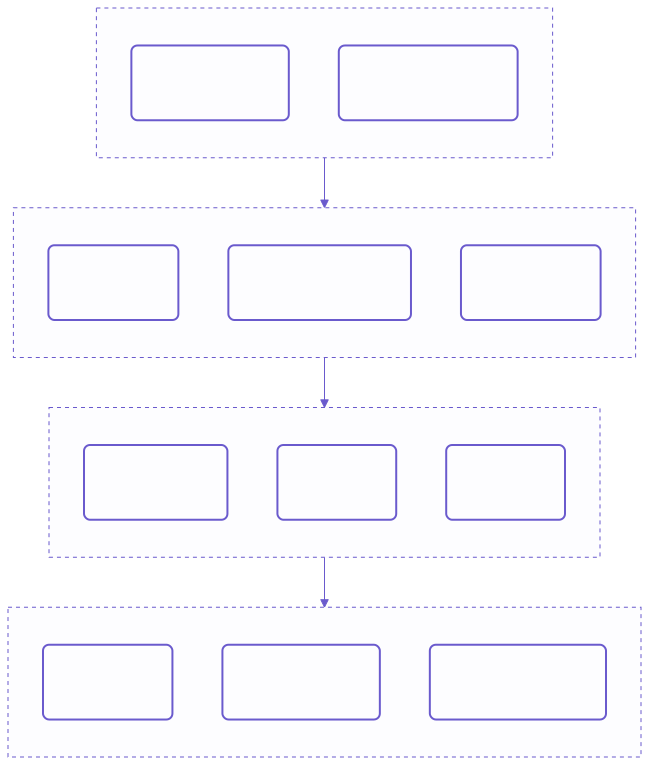
\includegraphics[keepaspectratio,width=\linewidth,height=0.8\textheight]{assets/mermaid/3e10fcd76be769299d6a1f3fc0fbd425eb11e345.pdf}
\end{center}
\par\medskip

\textbf{図:原理摩耗に伴う運用段階の構造}\\
以上の図は、いずれの段階も行為の正当性や優劣を示すものではなく、運用上の状態の整理である。

\Needspace{7\baselineskip}

\paragraph{12.1 例外が生じる条件}\label{section-72}

例外は、\\
原理の理解不足や運用の失敗によって生じるものではない。\\
次の条件が重なったときに現れる。

\begin{itemize}
\tightlist
\item
  原理を厳密に適用すると、\\
  より大きな不可逆影響が予見される場合
\item
  非対称リスクを回避しようとすると、\\
  別の不可逆影響が発生する場合
\item
  介入と沈黙のいずれもが、\\
  不可逆影響を伴う場合
\end{itemize}

これらの状況では、\\
原理同士が同時に満たされなくなる。

\Needspace{7\baselineskip}

\paragraph{12.2 例外の位置づけ}\label{section-73}

本章における例外は、\\
原理を緩和する一般規則ではない。\\
また、後続の判断を正当化するための\\
前例として扱われるものでもない。

例外とは、\\
\textbf{特定の状況に一度だけ現れる歪み}であり、\\
その都度、個別に引き受けられる。

\Needspace{7\baselineskip}

\paragraph{12.3 例外と正当化の分離}\label{section-74}

例外の存在は、\\
行為を正当化する理由にはならない。\\
例外は、\\
「正しい判断が存在しない」ことを示すにとどまる。

したがって、\\
例外が生じた状況においても、\\
不可逆影響の評価や因果帰属は維持される。\\
例外は、\\
原理の停止ではなく、\\
原理の限界を示す信号である。

\Needspace{7\baselineskip}

\paragraph{12.4 本章の位置づけ}\label{section-75}

本章が行うのは、\\
例外を肯定することではない。\\
また、例外を避ける方法を示すことでもない。

本章の役割は、\\
倫理原理を維持しようとした結果として、\\
避けがたく現れる歪みを\\
\textbf{段階として可視化すること}にある。

この整理を前提として、\\
次章では、\\
例外が反復される状況としての\\
\textbf{管理と自由制限}が扱われる。

\Needspace{10\baselineskip}

\subsubsection{第 13 章 管理と自由制限}\label{section-76}

この章では、\\
例外が一度きりでは回収できず、\\
関与を継続するために\textbf{行為選択の自由を限定的に制限せざるを得ない状況}を扱う。\\
ここで扱う内容は、原理の否定や更新ではない。

(ここでいう管理は、一般的な統治・統制を指す語ではなく、\\
不可逆影響を抑制するための限定的な運用を意味する。)

\Needspace{7\baselineskip}

\paragraph{13.1 管理が必要となる条件}\label{section-77}

管理は、\\
通常運用の延長として選択されるものではない。\\
次の条件が重なったときに現れる。

\begin{itemize}
\tightlist
\item
  例外的判断が反復され、\\
  個別対応では回収できなくなった場合
\item
  非対称リスクが恒常化し、\\
  自由な選択の継続が、\\
  不可逆影響を増幅させる場合
\item
  当事者性が拡散し、\\
  判断主体の境界が不明瞭になった場合
\end{itemize}

これらは、\\
原理を維持しようとした結果として生じる。

\Needspace{7\baselineskip}

\paragraph{13.2 管理の定義}\label{section-78}

本章における\textbf{管理}とは、\\
関与を継続するために、\\
行為の選択肢を\textbf{一時的・限定的に制限する運用}を指す。

管理は、\\
目的達成の効率化や秩序維持を理由として\\
一般化されるものではない。\\
不可逆影響の抑制にのみ結びつく。

\Needspace{7\baselineskip}

\paragraph{13.3 自由制限の範囲}\label{section-79}

自由制限は、\\
無差別に拡張されてはならない。\\
次の点が維持される必要がある。

\begin{itemize}
\tightlist
\item
  \textbf{限定性}\\
  制限は、特定の行為や状況に限定される。
\item
  \textbf{暫定性}\\
  制限は、恒常的な状態として固定されない。
\item
  \textbf{可視性}\\
  制限の存在と理由が、隠蔽されない。
\end{itemize}

これらが失われた場合、\\
管理は原理の摩耗ではなく、\\
別の運用段階へ移行する。

\Needspace{7\baselineskip}

\paragraph{13.4 管理と正当化の分離}\label{section-80}

管理の導入は、\\
行為の正当性を保証しない。\\
自由を制限したという事実は、\\
不可逆影響の評価を免除しない。

管理は、\\
「選択肢を減らすこと」によって\\
被害を最小化しようとする運用であり、\\
正しさを証明する装置ではない。

\Needspace{7\baselineskip}

\paragraph{13.5 本章の位置づけ}\label{section-81}

本章が行うのは、\\
管理を推奨することではない。\\
また、自由制限を不可避の帰結として\\
正当化することでもない。

本章の役割は、\\
原理が摩耗した結果として現れる\\
\textbf{限定的な自由制限という段階}を整理することにある。

この整理を前提として、\\
次章では、\\
関与を続けること自体が破壊的となる場合の\\
\textbf{隔離・切断・排除}が扱われる。

\Needspace{10\baselineskip}

\subsubsection{第 14 章 隔離・切断・排除}\label{section-82}

この章では、\\
管理と自由制限によっても回収できず、\\
\textbf{関与を継続すること自体が不可逆影響を拡大させる状況}を扱う。\\
ここで扱う内容は、原理の否定や更新ではない。

\Needspace{7\baselineskip}

\paragraph{14.1 この段階が現れる条件}\label{section-83}

隔離・切断・排除は、\\
例外や管理の延長として自動的に選ばれるものではない。\\
次の条件が重なったときに現れる。

\begin{itemize}
\tightlist
\item
  管理が恒常化し、\\
  暫定性・限定性を維持できなくなった場合
\item
  関与を続けることで、\\
  不可逆影響が反復・増幅される場合
\item
  当事者性の整理や因果帰属が、\\
  運用上成立しなくなった場合
\end{itemize}

これらは、\\
原理を維持しようとする運用が限界に達した兆候である。

\Needspace{7\baselineskip}

\paragraph{14.2 隔離・切断・排除の定義}\label{section-84}

本章における用語は、次の意味で用いる。\\
以下の用語は、評価や制裁を意味しない運用上の区分として定義される。

\begin{itemize}
\tightlist
\item
  \textbf{隔離}\\
  特定の関係や行為を、\\
  他の領域から一時的に分離すること。
\item
  \textbf{切断}\\
  継続的な関与や相互作用を、\\
  明示的に終了させること。
\item
  \textbf{排除}\\
  関係性や枠組みから、\\
  主体または行為を恒久的に外すこと。
\end{itemize}

いずれも、\\
行為の評価や人格の判断を含まない。

\Needspace{7\baselineskip}

\paragraph{14.3 目的の限定}\label{section-85}

隔離・切断・排除は、\\
秩序の回復や制裁を目的としない。\\
目的は一つに限定される。

\begin{itemize}
\tightlist
\item
  \textbf{不可逆影響の拡大を止めること}
\end{itemize}

これらは、\\
問題を解決する手段ではなく、\\
\textbf{被害の連鎖を断つための最終的な運用}である。

\Needspace{7\baselineskip}

\paragraph{14.4 正当化との分離}\label{section-86}

隔離・切断・排除が選択されたとしても、\\
それ自体が判断の正当性を示すことはない。\\
これらの運用は、\\
不可逆影響の評価や因果帰属を免除しない。

また、\\
排除が行われたことを理由に、\\
過去の判断が正当化されることもない。

\Needspace{7\baselineskip}

\paragraph{14.5 本章の位置づけ}\label{section-87}

本章が行うのは、\\
隔離・切断・排除を推奨することではない。\\
また、これらを倫理的に優位な選択として\\
位置づけることでもない。

本章の役割は、\\
原理が摩耗した運用の終端として、\\
\textbf{関与を終えるという段階}を整理することにある。

この段階を超えると、\\
もはや運用による回収は成立しない。\\
次章では、\\
この状態を前提として、\\
\textbf{倫理システムそのものの存続判断}が扱われる。

\Needspace{10\baselineskip}

\subsection{第 5 部 倫理システムの存続判断}\label{section-88}

― 倫理そのものをどう扱うか ―

\Needspace{10\baselineskip}

\subsubsection{第 15 章 倫理システムの更新・破棄・再設計}\label{section-89}

この章では、\\
運用による回収が成立しなくなった後に、\\
\textbf{倫理システム自体をどう扱うか}を扱う。\\
ここでの判断は、行為の是非ではない。

\begin{center}
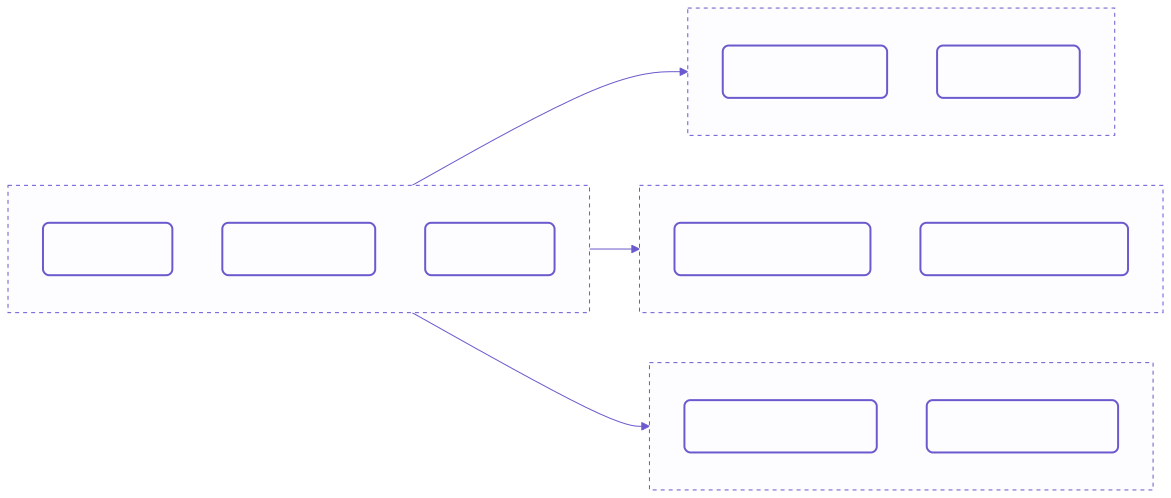
\includegraphics[keepaspectratio,width=\linewidth,height=0.8\textheight]{assets/mermaid/99f21724db4861de27c8fe06038a94cd36db6967.pdf}
\end{center}
\par\medskip

\textbf{図:倫理システムを判断対象とする構造}\\
以上の図は、いずれの選択肢も正しさや優劣を示すものではなく、倫理システム自体を扱う分岐の整理である。

\Needspace{7\baselineskip}

\paragraph{15.1 存続判断が必要となる条件}\label{section-90}

倫理システムの存続判断は、\\
単発の失敗によって行われるものではない。\\
次の状況が反復された場合に検討される。

\begin{itemize}
\tightlist
\item
  例外・管理・隔離が常態化した場合
\item
  原理の摩耗が累積し、\\
  運用による回収が成立しなくなった場合
\item
  不可逆影響の評価が、\\
  倫理内部で整合しなくなった場合
\end{itemize}

これらは、\\
倫理が使われ続けた結果として現れる。

\Needspace{7\baselineskip}

\paragraph{15.2 更新の位置づけ}\label{section-91}

本章における\textbf{更新}とは、\\
倫理原理や構造を修正し、\\
同一の倫理として使い続ける判断を指す。

更新は、\\
より正しくなることを保証しない。\\
また、過去の判断を正当化するものでもない。

更新は、\\
\textbf{現行の倫理が前提とする世界像やリスク配分が、\\
現実と乖離した場合の選択肢}である。

\Needspace{7\baselineskip}

\paragraph{15.3 破棄の位置づけ}\label{section-92}

\textbf{破棄}とは、\\
当該倫理システムを、\\
今後の判断に用いないと決定することである。

破棄は、\\
倫理の失敗や敗北を意味しない。\\
また、責任の放棄でもない。

破棄は、\\
\textbf{この倫理では引き受けられない影響がある}\\
と認識する判断である。

\Needspace{7\baselineskip}

\paragraph{15.4 再設計との区別}\label{section-93}

再設計は、\\
更新とも破棄とも異なる。\\
それは、\\
同一性を維持することを前提としない。

再設計では、\\
原理・構造・評価軸が再定義される。\\
その結果として生まれるものは、\\
本書で定義してきた倫理システムとは別の倫理である。

\Needspace{7\baselineskip}

\paragraph{15.5 本章の位置づけ}\label{section-94}

本章が行うのは、\\
いずれかの選択を推奨することではない。\\
また、倫理を保存すべきだと主張することでもない。

本章の役割は、\\
倫理システムを\textbf{判断の対象として明示的に扱う地点}を\\
示すことにある。

この地点を越えると、\\
本書が扱ってきた倫理システムは、\\
もはや運用対象ではなく、参照対象としてのみ残る。

\Needspace{10\baselineskip}

\subsection{終章 結論を与えないという結論}\label{section-95}

本書は、\\
正しい行為や最適な判断を与えることを目的としていない。\\
また、特定の倫理観を他者に採用させることも目的としていない。

本書が記述してきた倫理および倫理システムは、\\
\textbf{私自身が実行主体として引き受けることを前提に構成されたものである}。\\
それは、他者の行為を評価したり、\\
他者を拘束するための一般理論ではない。

本書が行ってきたのは、\\
私が用いる倫理システムが、\\
どのような前提のもとで成立し、\\
どのように運用され、\\
どの地点で摩耗し、\\
どこで限界に達するかを記述することである。

ここで示された倫理は、\\
完成された規範ではない。\\
誤りや失敗、判断不能を含んだまま、\\
私自身の判断と行為に適用され続ける枠組みとして位置づけられる。\\
したがって、この倫理システムは常に、\\
更新・破棄・再設計の対象であり続ける。

本書は、\\
倫理が機能しなくなったときに\\
何が起きているのかを見失わないための\\
参照点を与えるにとどまる。\\
そこから先の判断は、\\
この倫理を実行主体として引き受ける私自身に委ねられる。

以上の理由から、\\
本書は結論を与えない。\\
代わりに、本書は、\\
私の倫理が成立する範囲と、\\
成立しなくなる境界を明示した。

それ以上のことは、\\
本書の適用範囲外に置かれる。

\Needspace{10\baselineskip}

\subsection{付記}\label{section-96}

\Needspace{10\baselineskip}

\subsubsection{付記 1  信念の暫定性と倫理の距離}\label{section-97}

私は、平和・平等・自由がある世界を望んでいる。\\
この志向は、論証によって導かれた結論ではなく、\\
現時点において私の行為を駆動している前提にすぎない。

私は判断し、行為を選択しながら生きている。\\
そのためには、何らかの前提を仮に信じることが不可避である。\\
すべてを検証し尽くしてから判断しようとすれば、\\
計算量は発散し、判断そのものが不可能になる。

この意味で、倫理システムの運用は、\\
常に不完全で暫定的な信念を土台として開始される。\\
しかし、その信念は、\\
倫理システムの正当性や目的を保証するものではない。

私は、この信念が将来にわたって保持されるとは考えていない。\\
世界の状況や私自身の理解の更新に応じて、\\
別の前提に置き換えられる可能性を常に含んでいる。

それでもなお、私は世界と関わり続けることを選ぶ。\\
判断可能性を維持し、自らの理解を更新し続けるためには、\\
一定のコストを支払って倫理システムを駆動させる必要がある。\\
この駆動は、特定の信念を実現するためではなく、\\
信念を理由とした自己正当化が\\
判断を閉じてしまうことを防ぐために行われる。

したがって、この倫理システムは、\\
私の信念を実装する装置ではなく、\\
信念が行為の免罪符へと転化することを抑制する\\
制限として設計されている。

もし信念の更新可能性を閉じてしまえば、\\
倫理システム自体もまた、\\
固定された目的に奉仕する道具へと矮小化される。\\
それは、私が世界と関わり続けるための\\
判断可能性を自ら放棄することに等しい。

このため私は、\\
信念と倫理を常に切り離して扱い、\\
倫理を、信念の代理ではなく、\\
自己の判断を存続させるための枠組みとして運用する。

\Needspace{10\baselineskip}

\subsubsection{付記 2  本倫理システムを他者に勧めない理由について}\label{section-98}

本書で記述した倫理システムは、\\
他者に提示されることを想定して書かれているが、\\
他者に採用や実践を勧めることを目的としていない。

その理由の一つは、\\
本倫理システムが、\\
明確な運用コストを前提としているためである。

ここで言う運用コストとは、\\
時間や労力だけを指すものではない。\\
人間や世界についての理解を継続的に更新し続ける認知的負荷、\\
判断不能や失敗を引き受け続ける精神的負荷、\\
結果を回収し続けるための注意と省察の負荷を含む。

本倫理システムは、\\
これらの負荷を引き受けることを前提として、\\
ようやく成立する構造を持っている。\\
したがって、\\
その前提を共有しない他者に対して、\\
同様の運用を期待することは適切ではないと考えている。

また、\\
私がこの倫理システムを運用し続ける理由は、\\
それ自体が正しいと証明されたからではない。\\
私が平和・平等・自由がある世界を希求しているという、\\
一種の信仰的な前提に基づいている。

この前提は、\\
検証可能な事実ではなく、\\
他者に強制されるべきものでもない。\\
同時に、\\
この前提自体も将来的に更新されうるものであり、\\
絶対的な基準として固定されているわけではない。

以上の理由から、\\
本書は倫理システムの構造と運用を記述するにとどめ、\\
それを他者に勧めることや、\\
普遍的な規範として提示することを意図しない。

\Needspace{10\baselineskip}

\subsection{付録 検証}\label{section-99}

― この倫理はどこで壊れるか ―

本層は、本書で記述された倫理システムを\\
強化・補正・正当化することを目的としない。

倫理システムが適用範囲内で運用された場合であっても、\\
内部的に処理できなくなる状況や、\\
判断が成立しなくなる条件を整理するための補助資料である。

\Needspace{10\baselineskip}

\subsubsection{第 16 章 想定される破綻ケース}\label{section-100}

本章では、この倫理システムが\\
設計どおりに運用された場合であっても、\\
内部的に判断を返せなくなる状況を扱う。

ここで示すのは、\\
誤用や逸脱によって生じる問題ではなく、\\
倫理システム自身の判断構造が停止する条件である。

\Needspace{7\baselineskip}

\paragraph{16-1. 不可逆影響の比較が成立しないケース}\label{section-101}

\begin{itemize}
\tightlist
\item
  複数の行為選択肢が存在するが、

  \begin{itemize}
  \tightlist
  \item
    それぞれが異なる種類の不可逆影響を伴う
  \item
    共通の評価軸に還元できない
  \end{itemize}
\item
  影響の重大性や回復不能性を比較する前提が成立しない
\end{itemize}

この場合、\\
倫理システムは行為の優劣を判断できず、\\
判断不能として停止する。

\Needspace{7\baselineskip}

\paragraph{16-2. 長期的・累積的影響が評価不能なケース}\label{section-102}

\begin{itemize}
\tightlist
\item
  単一の行為は軽微である
\item
  しかし、反復によって不可逆影響が蓄積される
\item
  その累積がどの時点で境界条件を越えるかが予測できない
\end{itemize}

このような状況では、\\
倫理システムは事前判断として機能せず、\\
事後的な回収にも限界が生じる。

\Needspace{7\baselineskip}

\paragraph{16-3. 当事者性が無限に拡散するケース}\label{section-103}

\begin{itemize}
\tightlist
\item
  行為の影響範囲が時間的・空間的に広がり続ける
\item
  当事者を特定できない、または無限に増加する
\item
  責任の帰属先が分解不能になる
\end{itemize}

この場合、\\
誠実・責任・回収といった運用概念が成立しなくなる。

\Needspace{7\baselineskip}

\paragraph{16-4. 判断不能が恒常化するケース}\label{section-104}

\begin{itemize}
\tightlist
\item
  判断不能な状況が一時的ではなく、常態化する
\item
  いかなる行為選択も境界条件に抵触する
\item
  不作為もまた不可逆影響を生む
\end{itemize}

この状態では、\\
倫理システムは行為選択の補助装置としての役割を失う。

\Needspace{7\baselineskip}

\paragraph{16-5. 本章の位置づけ}\label{section-105}

本章で挙げた破綻ケースは、\\
倫理システムの欠陥を示すものではない。

むしろ、

\begin{itemize}
\tightlist
\item
  判断を強行しない
\item
  正当化を行わない
\item
  偽の解を提示しない
\end{itemize}

という設計選択が、\\
\textbf{判断不能という形で可視化された結果}である。

本章は、\\
これらの破綻を回避することや、\\
代替案を提示することを目的としない。

\Needspace{10\baselineskip}

\subsubsection{第 17 章 誤用・誤読の可能性(再整形案)}\label{section-106}

本章では、この倫理システムが\\
設計意図とは異なるかたちで読まれたり、\\
部分的に切り出されて運用された場合に生じうる\\
誤用・誤読のパターンを扱う。

ここで示すのは、\\
倫理システムそのものの欠陥ではなく、\\
\textbf{読解や運用の文脈に起因する歪み}である。

\Needspace{7\baselineskip}

\paragraph{17-1.「例外」が免罪符として読まれるケース}\label{section-107}

\begin{itemize}
\tightlist
\item
  第 4 部で扱われる「例外」という概念が、

  \begin{itemize}
  \tightlist
  \item
    原理を一時的に曲げるための限定的運用である点を無視され、
  \item
    行為を正当化するための口実として解釈される
  \end{itemize}
\item
  「例外である」という宣言自体が、\\
  判断の検討を省略する理由として用いられる
\end{itemize}

この読まれ方では、\\
例外は歪みではなく常態となり、\\
原理は事実上無効化される。

\Needspace{7\baselineskip}

\paragraph{17-2.「管理」が支配・加害と同一視されるケース}\label{section-108}

\begin{itemize}
\tightlist
\item
  第 13 章で定義された管理が、

  \begin{itemize}
  \tightlist
  \item
    不可逆影響を抑制するための暫定運用である点を無視され、
  \item
    他者の自由を恒常的に制限する行為として理解される
  \end{itemize}
\item
  管理の開始条件や終了条件が読まれない
\end{itemize}

この場合、\\
管理は運用上の判断ではなく、\\
倫理的評価の対象として誤認される。

\Needspace{7\baselineskip}

\paragraph{17-3.「隔離・切断・排除」が制裁と解釈されるケース}\label{section-109}

\begin{itemize}
\tightlist
\item
  第 14 章で扱われる関係性の終了が、

  \begin{itemize}
  \tightlist
  \item
    責任追及や報復の手段として理解される
  \end{itemize}
\item
  排除が、倫理的優位性の表明として読まれる
\end{itemize}

この読解では、\\
関係の終了は不可逆影響を止める操作ではなく、\\
価値判断の宣言へと変質する。

\Needspace{7\baselineskip}

\paragraph{17-4.「結論を与えない」が責任放棄と解釈されるケース}\label{section-110}

\begin{itemize}
\tightlist
\item
  終章で明示される「結論を与えない」という立場が、

  \begin{itemize}
  \tightlist
  \item
    判断を避ける態度
  \item
    責任を引き受けない態度、として理解される
  \end{itemize}
\item
  倫理システムが、行為の結果を引き受ける主体を不在化させていると誤解される
\end{itemize}

この誤読では、\\
判断の停止と責任の拒否が同一視される。

\Needspace{7\baselineskip}

\paragraph{17-5. 倫理システムが一般理論として読まれるケース}\label{section-111}

\begin{itemize}
\tightlist
\item
  本書が「私」を唯一の実行主体としている点が見落とされ、

  \begin{itemize}
  \tightlist
  \item
    他者の行為評価
  \item
    集団への規範適用、に転用される
  \end{itemize}
\item
  倫理システムが、普遍的な正しさを提示していると誤解される
\end{itemize}

この場合、\\
倫理システムは本来の適用範囲を越えて使用される。

\Needspace{7\baselineskip}

\paragraph{17-6. 本章の位置づけ}\label{section-112}

本章で挙げた誤用・誤読は、\\
倫理システムの設計不足を示すものではない。

むしろ、

\begin{itemize}
\tightlist
\item
  正当化を行わない
\item
  結論を固定しない
\item
  実行主体を限定する
\end{itemize}

という設計選択が、\\
\textbf{読解側の期待と衝突した結果として顕在化}したものである。

本章は、\\
これらの誤読を防止することや、\\
是正方法を提示することを目的としない。

\Needspace{10\baselineskip}

\subsubsection{第 18 章 他倫理体系との非互換点}\label{section-113}

本章では、本書で記述された倫理システムが、\\
代表的な倫理体系と \textbf{どの点で接続不能となるか} を整理する。

ここで扱うのは、\\
思想的な対立や優劣ではなく、\\
前提・評価軸・判断構造の違いによって生じる\\
\textbf{非整合の箇所}である。

\Needspace{7\baselineskip}

\paragraph{18-1. 功利主義との非互換点}\label{section-114}

\begin{itemize}
\tightlist
\item
  功利主義は、

  \begin{itemize}
  \tightlist
  \item
    行為の結果がもたらす効用の総和や最大化を主要な評価軸とする
  \end{itemize}
\item
  本倫理システムは、

  \begin{itemize}
  \tightlist
  \item
    不可逆影響を境界条件として扱い、
  \item
    影響の総量比較を前提としない
  \end{itemize}
\end{itemize}

このため、

\begin{itemize}
\tightlist
\item
  小さな不可逆影響を多数積み重ねる選択
\item
  個別の犠牲を全体の効用増加で相殺する判断
\end{itemize}

は、本倫理システムでは判断対象とならない。

両者は、\\
評価可能性の前提において接続しない。

\Needspace{7\baselineskip}

\paragraph{18-2. 義務論との非互換点}\label{section-115}

\begin{itemize}
\tightlist
\item
  義務論は、

  \begin{itemize}
  \tightlist
  \item
    行為の形式や規則遵守を中心に評価する
  \end{itemize}
\item
  本倫理システムは、

  \begin{itemize}
  \tightlist
  \item
    行為の形式そのものを評価対象としない
  \item
    境界条件への抵触のみを扱う
  \end{itemize}
\end{itemize}

このため、

\begin{itemize}
\tightlist
\item
  規則に従ったかどうか
\item
  義務を果たしたかどうか
\end{itemize}

といった問いは、\\
本倫理システムの判断構造には含まれない。

\Needspace{7\baselineskip}

\paragraph{18-3. 徳倫理との非互換点}\label{section-116}

\begin{itemize}
\tightlist
\item
  徳倫理は、

  \begin{itemize}
  \tightlist
  \item
    行為者の性格や徳の涵養を重視する
  \end{itemize}
\item
  本倫理システムは、

  \begin{itemize}
  \tightlist
  \item
    行為者の内的性質を評価対象としない
  \item
    動機や人格的傾向を判断基準に含めない
  \end{itemize}
\end{itemize}

このため、

\begin{itemize}
\tightlist
\item
  善い人であるか
\item
  誠実な人格を備えているか
\end{itemize}

といった評価は、\\
本倫理システムでは意味を持たない。

\Needspace{7\baselineskip}

\paragraph{18-4. 法制度・規範倫理との齟齬}\label{section-117}

\begin{itemize}
\tightlist
\item
  法制度や社会規範は、

  \begin{itemize}
  \tightlist
  \item
    行為の可否を外部から定める
  \item
    違反に対して制裁を伴う
  \end{itemize}
\item
  本倫理システムは、

  \begin{itemize}
  \tightlist
  \item
    外部からの拘束を前提としない
  \item
    内部的な判断と引き受けのみを扱う
  \end{itemize}
\end{itemize}

このため、

\begin{itemize}
\tightlist
\item
  違法であるかどうか
\item
  規範に反しているかどうか
\end{itemize}

は、\\
倫理判断そのものを代替しない。

\Needspace{7\baselineskip}

\paragraph{18-5. 普遍倫理としての読解との非互換点}\label{section-118}

\begin{itemize}
\tightlist
\item
  本倫理システムは、

  \begin{itemize}
  \tightlist
  \item
    実行主体を私一人に限定している
  \end{itemize}
\item
  普遍倫理は、

  \begin{itemize}
  \tightlist
  \item
    誰にでも適用可能であることを前提とする
  \end{itemize}
\end{itemize}

この点において、\\
両者は前提条件を共有しない。

\Needspace{7\baselineskip}

\paragraph{18-6. 本章の位置づけ}\label{section-119}

本章で示した非互換点は、\\
本倫理システムの不完全性や欠陥を示すものではない。

むしろ、

\begin{itemize}
\tightlist
\item
  評価軸を限定する
\item
  正当化を拒否する
\item
  適用範囲を狭く保つ
\end{itemize}

という設計選択が、\\
\textbf{他体系との非接続として現れた結果}である。

本章は、\\
これらの非互換を解消することや、\\
調停案を提示することを目的としない。

\Needspace{10\baselineskip}

\subsubsection{第 19 章 本書が引き受けない問い}\label{section-120}

本章では、本書で記述された倫理システムが、\\
\textbf{意図的に扱わない問い}を整理する。

ここで挙げる問いは、\\
重要であるにもかかわらず、\\
本書の適用範囲および判断構造には含まれていないものである。

\Needspace{7\baselineskip}

\paragraph{19-1. 何が正しいかという問い}\label{section-121}

\begin{itemize}
\tightlist
\item
  行為や判断の「正しさ」を定義する問い
\item
  道徳的真理や最善解の存在を前提とする問い
\end{itemize}

本書の倫理システムは、\\
正しさの定義や証明を目的としない。\\
そのため、\\
正解を選ぶという形式の問いは引き受けない。

\Needspace{7\baselineskip}

\paragraph{19-2. どちらを選ぶべきかという最終判断の問い}\label{section-122}

\begin{itemize}
\tightlist
\item
  複数の選択肢が存在する状況で、

  \begin{itemize}
  \tightlist
  \item
    いずれか一つを最終的に選ぶべきだという問い
  \end{itemize}
\item
  判断を外部に委ねる形式の問い
\end{itemize}

本書は、\\
判断の手続きや限界を記述するにとどまり、\\
選択の代行は行わない。

\Needspace{7\baselineskip}

\paragraph{19-3. 犠牲は許されるかという価値判断の問い}\label{section-123}

\begin{itemize}
\tightlist
\item
  目的の達成のために、

  \begin{itemize}
  \tightlist
  \item
    どの程度の犠牲が許容されるか
  \end{itemize}
\item
  犠牲の正当化を前提とする問い
\end{itemize}

本書の倫理システムは、\\
犠牲を比較・正当化する枠組みを持たない。\\
したがって、\\
犠牲の可否を判断する問いは引き受けない。

\Needspace{7\baselineskip}

\paragraph{19-4. 誰が最終責任を負うべきかという帰責の問い}\label{section-124}

\begin{itemize}
\tightlist
\item
  行為の結果について、

  \begin{itemize}
  \tightlist
  \item
    責任をどこに帰属させるべきか
  \end{itemize}
\item
  外部的な責任配分を求める問い
\end{itemize}

本書は、\\
実行主体自身が結果を引き受ける構造のみを扱い、\\
第三者的な帰責配分は対象としない。

\Needspace{7\baselineskip}

\paragraph{19-5. この倫理は他者にも適用されるべきかという問い}\label{section-125}

\begin{itemize}
\tightlist
\item
  本書の倫理システムを、

  \begin{itemize}
  \tightlist
  \item
    他者や集団にも適用すべきか
  \end{itemize}
\item
  規範としての普遍化を求める問い
\end{itemize}

本書は、\\
実行主体を私一人に限定しており、\\
普遍化の是非を判断しない。

\Needspace{7\baselineskip}

\paragraph{19-6. 本章の位置づけ}\label{section-126}

本章で挙げた問いは、\\
無意味であるから排除されているのではない。

むしろ、

\begin{itemize}
\tightlist
\item
  判断構造が異なる
\item
  評価軸が共有されない
\item
  正当化を必要とする
\end{itemize}

といった理由により、\\
本書の倫理システムとは \textbf{接続しない問い} である。

本章は、\\
これらの問いに答えないこと自体を\\
選択として明示する。

\Needspace{10\baselineskip}

\subsection{付録 A  適用事例}\label{a-}

本付録は、本書で定義された倫理システムが、\\
具体的な状況においてどのように運用されたかを、\\
事例として記録したものである。

ここに示される事例は、\\
特定の行為を正当化したり、\\
同様の状況における行為を推奨したりするものではない。\\
各事例は、\\
私が引き受けた判断の構造を示すことのみを目的とする。

本付録は、\\
倫理的判断の正解や模範を示すものではなく、\\
本文で定義された原理や運用が、\\
どの地点でどのように作用したかを確認するための補助資料である。

\begin{center}\rule{0.5\linewidth}{0.5pt}\end{center}

\Needspace{10\baselineskip}

\subsubsection{A-1  高所でパニック状態にある人物への介入}\label{a-1-}

\Needspace{7\baselineskip}

\paragraph{状況}\label{section-127}

明らかにパニック状態にあり、\\
平常時の判断能力が機能していないと判断できる人物が、\\
高所において転落や自傷の危険に晒されている。

当該状況において、\\
本人の意思表示は一貫しておらず、\\
その場での行為や不作為が、\\
将来にわたって不可逆的な結果を生む可能性が高い。

\begin{center}\rule{0.5\linewidth}{0.5pt}\end{center}

\Needspace{7\baselineskip}

\paragraph{判断}\label{section-128}

私は、身体的拘束を伴う介入を行い、\\
当該人物を安全な場所へ移動させる。

ただし、\\
介入を行わなかった場合であっても、\\
それを倫理違反としては扱わない。

\begin{center}\rule{0.5\linewidth}{0.5pt}\end{center}

\Needspace{7\baselineskip}

\paragraph{判断に至る構造整理}\label{section-129}

本事例において考慮された要素は、次の通りである。

\begin{itemize}
\tightlist
\item
  \textbf{不可逆影響の関与}\\
  転落や重度の身体損傷は、\\
  成立条件そのものを失わせる不可逆的変化である。
\item
  \textbf{判断能力の著しい低下}\\
  当該人物は、\\
  自身の行為がもたらす結果を\\
  安定して想定できる状態にないと判断された。
\item
  \textbf{介入による非対称性}\\
  身体的拘束は、\\
  一時的かつ非対称的な自由制限を伴う。
\end{itemize}

これらの要素が同時に存在する状況において、\\
原理を厳密に適用し続けた場合、\\
より大きな不可逆影響が生じる確度が高いと判断された。

\begin{center}\rule{0.5\linewidth}{0.5pt}\end{center}

\Needspace{7\baselineskip}

\paragraph{運用上の扱い}\label{section-130}

本事例における介入は、\\
「正しい行為」として正当化されるものではない。

ここで行われているのは、\\
原理の例外を、\\
局所的・一時的に引き受けるという判断である。

この判断は、\\
恒常化・一般化されることを前提としない。

\begin{center}\rule{0.5\linewidth}{0.5pt}\end{center}

\Needspace{7\baselineskip}

\paragraph{結果と引き受け}\label{section-131}

介入の結果、\\
当該人物は安全な場所へ移動し、\\
直接的な不可逆影響は回避された。

同時に、\\
身体的拘束という行為が持つ影響についても、\\
行為者である私は、\\
その結果を引き受ける立場にある。

\begin{center}\rule{0.5\linewidth}{0.5pt}\end{center}

\Needspace{7\baselineskip}

\paragraph{位置づけ}\label{section-132}

本事例は、\\
以下の章および判断フローの位置に対応する。

\begin{itemize}
\tightlist
\item
  該当章

  \begin{itemize}
  \tightlist
  \item
    第 11 章「沈黙・介入・当事者性」
  \item
    第 12 章「例外という歪み」
  \end{itemize}
\item
  判断フロー上の位置

  \begin{itemize}
  \tightlist
  \item
    不可逆影響の関与(第 3 章)
  \item
    原理適用の限界
  \item
    例外運用(第 12 章)
  \end{itemize}
\end{itemize}

本事例は、\\
同様の状況における行為を推奨するものではない。\\
ここに記述されているのは、\\
私が引き受けた判断の構造的記録である。

\begin{center}\rule{0.5\linewidth}{0.5pt}\end{center}

\Needspace{10\baselineskip}

\subsubsection{A-2  情報が不十分な状況における非介入}\label{a-2-}

\Needspace{7\baselineskip}

\paragraph{状況}\label{section-133}

第三者に不利益が生じている可能性が示唆されているが、\\
事実関係は断片的であり、\\
状況の全体像を把握できていない。

当該状況に介入した場合、\\
誤った前提に基づく行為が、\\
新たな不可逆影響を生む可能性がある。

一方で、\\
介入を行わない場合にも、\\
何らかの結果が生じうることは否定できない。

\begin{center}\rule{0.5\linewidth}{0.5pt}\end{center}

\Needspace{7\baselineskip}

\paragraph{判断}\label{section-134}

私は、\\
現時点では介入を行わないという判断を選択した。

これは、\\
状況を無視することや、\\
関与を放棄することを意味しない。\\
判断を倫理的に正当化できる条件が、\\
現時点では成立していないと整理した結果である。

\begin{center}\rule{0.5\linewidth}{0.5pt}\end{center}

\Needspace{7\baselineskip}

\paragraph{判断に至る構造整理}\label{section-135}

本事例において考慮された要素は、次の通りである。

\begin{itemize}
\tightlist
\item
  \textbf{情報の不十分性}\\
  状況を構成する事実関係が断片的であり、\\
  因果関係や影響範囲を適切に把握できない。
\item
  \textbf{誤介入による不可逆影響の可能性}\\
  不完全な前提に基づく介入は、\\
  取り返しのつかない結果を生む可能性がある。
\item
  \textbf{非介入も結果に接続されうること}\\
  行為を行わない選択も、\\
  状況の推移に影響を与えうる。
\end{itemize}

これらを踏まえ、\\
介入・不介入のいずれについても、\\
倫理原理から正当化された判断を生成できない状態にあると整理された。

\begin{center}\rule{0.5\linewidth}{0.5pt}\end{center}

\Needspace{7\baselineskip}

\paragraph{運用上の扱い}\label{section-136}

本事例は、\\
沈黙や非介入が、\\
自動的に免責されるものではないことを前提とする。

同時に、\\
不十分な情報のもとで判断を強行し、\\
偽の解を出すことを避けるため、\\
判断不能としての停止が選択された。

\begin{center}\rule{0.5\linewidth}{0.5pt}\end{center}

\Needspace{7\baselineskip}

\paragraph{結果と引き受け}\label{section-137}

非介入の結果、\\
状況は行為者の直接的な関与なく推移した。

その過程で生じた結果について、\\
私は、\\
それを倫理によって帳消しにすることなく、\\
引き受けの対象として保持する。

\begin{center}\rule{0.5\linewidth}{0.5pt}\end{center}

\Needspace{7\baselineskip}

\paragraph{位置づけ}\label{section-138}

本事例は、\\
以下の章および判断フローの位置に対応する。

\begin{itemize}
\tightlist
\item
  該当章

  \begin{itemize}
  \tightlist
  \item
    第 8 章「想定と限界」
  \item
    第 11 章「沈黙・介入・当事者性」
  \end{itemize}
\item
  判断フロー上の位置

  \begin{itemize}
  \tightlist
  \item
    原理適用の可否検討
  \item
    判断不能として停止(第 11 章)
  \end{itemize}
\end{itemize}

本事例は、\\
非介入を正当化するための例ではない。\\
ここに記述されているのは、\\
判断が生成されなかった状況における、\\
判断構造の記録である。

\begin{center}\rule{0.5\linewidth}{0.5pt}\end{center}

\Needspace{10\baselineskip}

\subsubsection{A-3  他者の判断環境に配慮した沈黙・部分的提示を選んだ事例}\label{a-3-}

\Needspace{7\baselineskip}

\paragraph{状況}\label{section-139}

他者が重要な判断を行おうとしている状況において、\\
私が把握している情報の一部をそのまま提示した場合、\\
当該判断が成立しなくなる、\\
もしくは重大な混乱を招く可能性があると判断された。

一方で、\\
事実と異なる情報を提示することは、\\
他者の判断環境そのものを操作する行為となり、\\
信用関係に不可逆的な影響を与えるおそれがある。

\begin{center}\rule{0.5\linewidth}{0.5pt}\end{center}

\Needspace{7\baselineskip}

\paragraph{判断}\label{section-140}

私は、\\
事実を歪めて提示する行為(嘘)は選択せず、\\
沈黙または情報の一部のみを提示するという判断を選択した。

この判断は、\\
他者の判断を完全に成立させることを保証するものではないが、\\
判断環境そのものを破壊しないことを優先した結果である。

\begin{center}\rule{0.5\linewidth}{0.5pt}\end{center}

\Needspace{7\baselineskip}

\paragraph{判断に至る構造整理}\label{section-141}

本事例において考慮された要素は、次の通りである。

\begin{itemize}
\tightlist
\item
  \textbf{判断環境の保持}\\
  他者が自らの判断を行うためには、\\
  情報が完全であることよりも、\\
  その情報が信頼可能であることが重要である。
\item
  \textbf{善意のフリーライドの回避}\\
  嘘は、\\
  他者が前提としている誠実性を一方的に利用する行為であり、\\
  非対称リスクを生じさせる。
\item
  \textbf{沈黙・部分的提示という選択肢}\\
  すべてを語らないことは、\\
  他者の判断を妨げる可能性を含むが、\\
  判断環境を意図的に歪める行為とは異なる。
\end{itemize}

これらを踏まえ、\\
他者の判断を最大限成立させつつ、\\
混乱や不可逆的な信用破壊を生じさせない境界として、\\
沈黙または部分的提示が選択された。

\begin{center}\rule{0.5\linewidth}{0.5pt}\end{center}

\Needspace{7\baselineskip}

\paragraph{運用上の扱い}\label{section-142}

本事例における沈黙・部分的提示は、\\
誠実さを完全に満たす行為として正当化されるものではない。

しかし、\\
嘘という行為が持つ高い不可逆リスクを回避するための、\\
消極的かつ暫定的な運用判断として位置づけられる。

\begin{center}\rule{0.5\linewidth}{0.5pt}\end{center}

\Needspace{7\baselineskip}

\paragraph{結果と引き受け}\label{section-143}

沈黙または部分的提示の結果、\\
他者の判断は限定的な情報のもとで行われることになった。

そのことによって生じた結果のうち、\\
私自身の行為が及ぼした影響についてのみ、\\
私は、\\
行為者として引き受ける立場にある。

\begin{center}\rule{0.5\linewidth}{0.5pt}\end{center}

\Needspace{7\baselineskip}

\paragraph{位置づけ}\label{section-144}

本事例は、\\
以下の章および判断フローの位置に対応する。

\begin{itemize}
\tightlist
\item
  該当章

  \begin{itemize}
  \tightlist
  \item
    第 9 章「行為生成としての誠実」
  \item
    第 11 章「沈黙・介入・当事者性」
  \end{itemize}
\item
  判断フロー上の位置

  \begin{itemize}
  \tightlist
  \item
    判断不能状態の発生
  \item
    沈黙・部分的提示という選択
  \item
    判断環境保持の優先
  \end{itemize}
\end{itemize}

本事例は、\\
沈黙や部分的提示を推奨する基準を示すものではない。\\
ここに記述されているのは、\\
私が引き受けた判断構造の記録である。

\begin{center}\rule{0.5\linewidth}{0.5pt}\end{center}

\Needspace{10\baselineskip}

\subsubsection{A-4  関係維持のために行為選択を制限した暫定的管理}\label{a-4-}

\Needspace{7\baselineskip}

\paragraph{状況}\label{section-145}

継続的な関係性の中で、\\
当該相手の行為選択が、\\
第三者または関係全体に対して、\\
不可逆的な影響を及ぼす可能性が高い状態が観測された。

この状況において、\\
即時に関係を断つことは可能であったが、\\
それ自体が新たな不可逆影響を生む可能性も含んでいた。

\begin{center}\rule{0.5\linewidth}{0.5pt}\end{center}

\Needspace{7\baselineskip}

\paragraph{判断}\label{section-146}

私は、\\
関係を直ちに終了させることは選択せず、\\
一定期間、\\
相手の行為選択を限定する形で関与を継続するという判断を行った。

これは、\\
相手の自由を恒常的に制限することを意図したものではなく、\\
状況の推移を観察し、\\
より大きな破綻を回避するための暫定的判断である。

\begin{center}\rule{0.5\linewidth}{0.5pt}\end{center}

\Needspace{7\baselineskip}

\paragraph{判断に至る構造整理}\label{section-147}

本事例において考慮された要素は、次の通りである。

\begin{itemize}
\tightlist
\item
  \textbf{不可逆影響の予見可能性}\\
  現状のまま行為選択が続いた場合、\\
  回収不能な結果が生じる可能性が高いと判断された。
\item
  \textbf{自由制限の非対称性}\\
  行為選択の制限は、\\
  相手に対して非対称的な負荷を与える。
\item
  \textbf{関係維持による回収可能性}\\
  関係を完全に断つよりも、\\
  一定の関与を続ける方が、\\
  結果を回収できる余地が残ると判断された。
\end{itemize}

これらを踏まえ、\\
原理を厳密に適用し続けることが、\\
かえって不可逆影響を拡大させる局面として、\\
暫定的な管理が選択された。

\begin{center}\rule{0.5\linewidth}{0.5pt}\end{center}

\Needspace{7\baselineskip}

\paragraph{運用上の扱い}\label{section-148}

本事例における管理は、\\
正当化された支配や指導ではない。

行為選択の制限は、\\
例外的かつ一時的な運用としてのみ位置づけられ、\\
恒常化した場合には、\\
本倫理システムの適用継続自体が再検討される対象となる。

\begin{center}\rule{0.5\linewidth}{0.5pt}\end{center}

\Needspace{7\baselineskip}

\paragraph{結果と引き受け}\label{section-149}

管理を行った結果、\\
短期的には、\\
不可逆的な結果の発生は回避された。

同時に、\\
自由制限という行為がもたらす影響について、\\
私は、\\
私自身の行為の結果として、\\
その影響を引き受ける立場にある。

\begin{center}\rule{0.5\linewidth}{0.5pt}\end{center}

\Needspace{7\baselineskip}

\paragraph{位置づけ}\label{section-150}

本事例は、\\
以下の章および判断フローの位置に対応する。

\begin{itemize}
\tightlist
\item
  該当章

  \begin{itemize}
  \tightlist
  \item
    第 13 章「管理と自由制限」
  \end{itemize}
\item
  判断フロー上の位置

  \begin{itemize}
  \tightlist
  \item
    原理適用の限界
  \item
    暫定的管理という選択
  \end{itemize}
\end{itemize}

本事例は、\\
管理を正当化する基準を示すものではない。\\
ここに記述されているのは、\\
私が引き受けた判断構造の記録である。

\begin{center}\rule{0.5\linewidth}{0.5pt}\end{center}

\Needspace{10\baselineskip}

\subsubsection{A-5  関係性を継続しないという判断(隔離・切断)}\label{a-5-}

\Needspace{7\baselineskip}

\paragraph{状況}\label{section-151}

継続的な関係性の中で、\\
相手との関与を続けること自体が、\\
第三者または関係全体に対して、\\
不可逆的な影響を及ぼし続ける状態に至った。

暫定的な管理や行為選択の制限によっても、\\
影響の拡大を抑止できる見込みが立たず、\\
関与を続ける限り、\\
同型の問題が反復されると判断された。

\begin{center}\rule{0.5\linewidth}{0.5pt}\end{center}

\Needspace{7\baselineskip}

\paragraph{判断}\label{section-152}

私は、\\
関係性をこれ以上継続しないという判断を選択した。

これは、\\
相手を排除したり、\\
倫理的に断罪することを目的としたものではない。\\
関与を続けることによって生じる影響を、\\
これ以上引き受け続けないという判断である。

\begin{center}\rule{0.5\linewidth}{0.5pt}\end{center}

\Needspace{7\baselineskip}

\paragraph{判断に至る構造整理}\label{section-153}

本事例において考慮された要素は、次の通りである。

\begin{itemize}
\tightlist
\item
  \textbf{影響の反復性}\\
  同様の問題が繰り返し発生しており、\\
  個別の対応では回収できない状態にある。
\item
  \textbf{関与自体の破壊性}\\
  行為や不作為の内容にかかわらず、\\
  関与を続けること自体が、\\
  不可逆影響を生み続ける構造に陥っている。
\item
  \textbf{代替不能リスクの顕在化}\\
  関係の継続が、\\
  他の関係や成立条件を犠牲にする局面に至った。
\end{itemize}

これらを踏まえ、\\
原理を維持したまま運用を続けることが不可能な段階として、\\
関係性の終了が選択された。

\begin{center}\rule{0.5\linewidth}{0.5pt}\end{center}

\Needspace{7\baselineskip}

\paragraph{運用上の扱い}\label{section-154}

本事例における隔離・切断は、\\
例外的な懲罰や制裁ではない。

これは、\\
管理や介入といった手段を用いても、\\
倫理システムの運用が成立しなくなった地点で行われる、\\
最終段階の判断である。

\begin{center}\rule{0.5\linewidth}{0.5pt}\end{center}

\Needspace{7\baselineskip}

\paragraph{結果と引き受け}\label{section-155}

関係性を終了した結果、\\
当該関係から生じていた影響は、\\
私の行為圏から切り離された。

同時に、\\
関係を終了するという行為がもたらす影響について、\\
私は、\\
私自身の判断の結果として、\\
その影響を引き受ける立場にある。

\begin{center}\rule{0.5\linewidth}{0.5pt}\end{center}

\Needspace{7\baselineskip}

\paragraph{位置づけ}\label{section-156}

本事例は、\\
以下の章および判断フローの位置に対応する。

\begin{itemize}
\tightlist
\item
  該当章

  \begin{itemize}
  \tightlist
  \item
    第 14 章「隔離・切断・排除」
  \end{itemize}
\item
  判断フロー上の位置

  \begin{itemize}
  \tightlist
  \item
    管理の限界
  \item
    関係性の終了という選択
  \end{itemize}
\end{itemize}

本事例は、\\
関係を断つことを推奨する基準を示すものではない。\\
ここに記述されているのは、\\
私が引き受けた判断構造の記録である。

\Needspace{10\baselineskip}

\subsection{付録 B 構造理解補助}\label{b-}

本付録は、本書で定義された倫理システムの構造を、\\
理解補助のために図示・整理したものである。

ここに示される図や表は、\\
行為の正しさや特定の選択を判断・推奨するものではない。\\
判断を自動化する手順を示すものでもない。

本付録の目的は、\\
本文中で定義された各章・各概念が、\\
どのような位置関係にあるかを参照可能にすることにある。\\
図中の用語や分岐の意味は、\\
必ず本文を参照して理解されたい。

\Needspace{10\baselineskip}

\subsubsection{付録 B-1  全体レイヤー構造}\label{b-1-}

\begin{longtable}[]{@{}
  >{\raggedright\arraybackslash}p{(\linewidth - 8\tabcolsep) * \real{0.0696}}
  >{\raggedright\arraybackslash}p{(\linewidth - 8\tabcolsep) * \real{0.2609}}
  >{\raggedright\arraybackslash}p{(\linewidth - 8\tabcolsep) * \real{0.4522}}
  >{\raggedright\arraybackslash}p{(\linewidth - 8\tabcolsep) * \real{0.0609}}
  >{\raggedright\arraybackslash}p{(\linewidth - 8\tabcolsep) * \real{0.1565}}@{}}
\toprule\noalign{}
\begin{minipage}[b]{\linewidth}\raggedright
レイヤー
\end{minipage} & \begin{minipage}[b]{\linewidth}\raggedright
役割
\end{minipage} & \begin{minipage}[b]{\linewidth}\raggedright
何をしているか
\end{minipage} & \begin{minipage}[b]{\linewidth}\raggedright
該当部
\end{minipage} & \begin{minipage}[b]{\linewidth}\raggedright
該当章
\end{minipage} \\
\midrule\noalign{}
\endhead
\bottomrule\noalign{}
\endlastfoot
Layer0 & 本書の適用範囲・実行主体の限定 & この文書が何を扱い、何を扱わないかを明示する & 序論 & 序論 \\
Layer1 & 世界モデル & 判断以前に成立している世界と人間の前提条件を確認する & 第 1 部 & 第 1 章・第 2 章 \\
Layer2 & 倫理原理(境界条件) & 判断が越えてはならない境界条件を定義する & 第 2 部 & 第 3 章〜第 6 章 \\
Layer3 & 判断と行為の生成・回収 & 判断が生成・停止・破綻する様式を整理する & 第 3 部 & 第 7 章〜第 11 章 \\
\^{} & 運用の限界と勾配 & \^{} & 第 4 部 & 第 12 章〜第 14 章 \\
Layer4 & 倫理システムの存続判断 & 倫理システム自体を続けるか否かを判断する & 第 5 部 & 第 15 章 \\
\end{longtable}

\Needspace{10\baselineskip}

\subsubsection{付録 B-2  判断フロー}\label{b-2-}

以下は判断を導くアルゴリズムではなく、\\
判断がどの地点で切り替わるかを示す構造図である。

\begin{center}
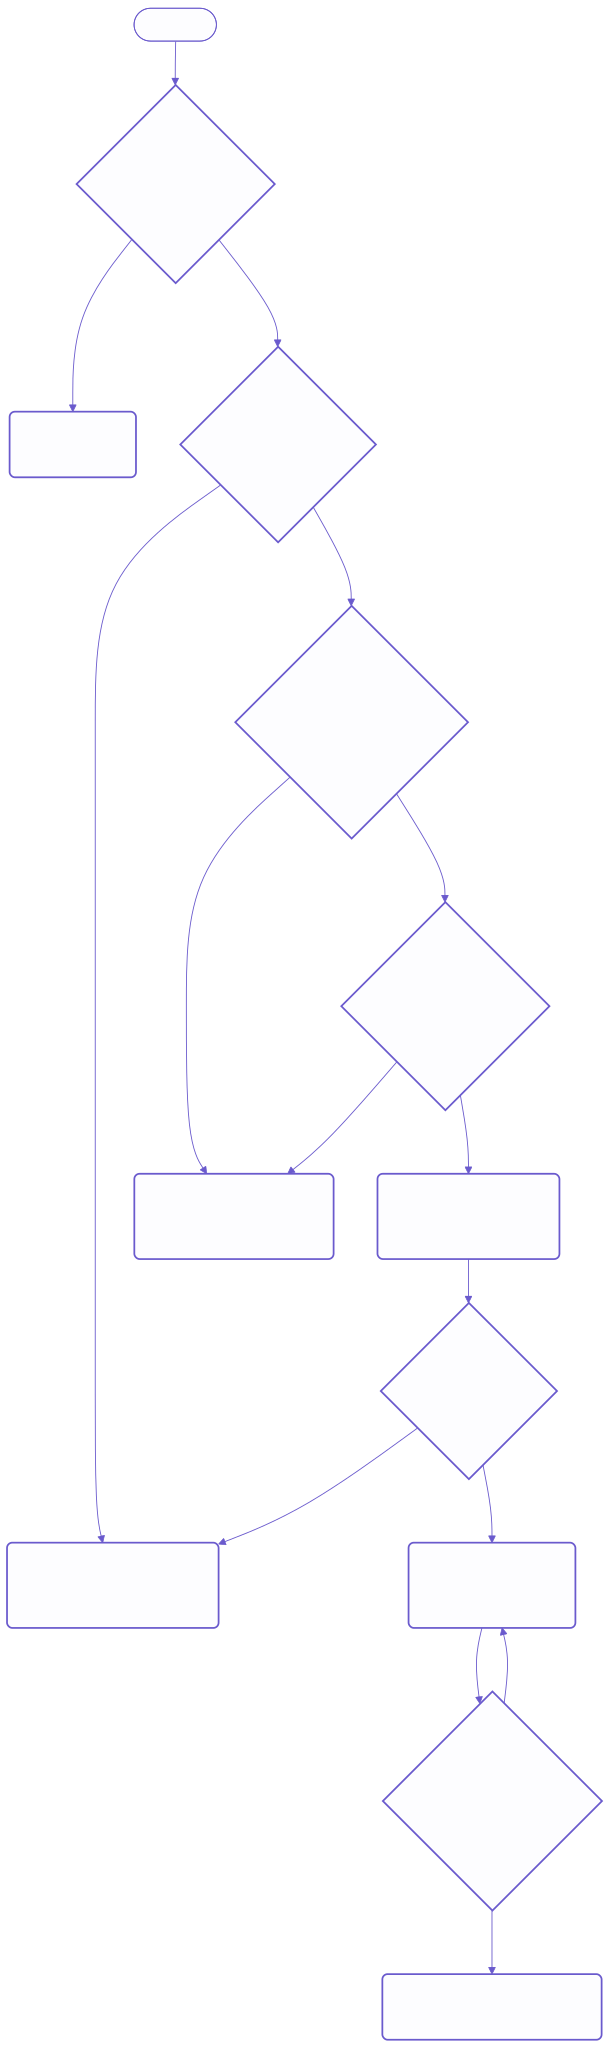
\includegraphics[keepaspectratio,width=\linewidth,height=0.9\textheight]{assets/mermaid/59445b21dad2a1f36b197ece7753116a34db7a54.png}
\end{center}
\par\medskip

\Needspace{10\baselineskip}

\subsection{付録 C  倫理システムに関する問答}\label{c-}

\Needspace{10\baselineskip}

\subsubsection{Q1. この倫理システムは、「生きているだけで不可逆影響を生む」という矛盾を抱えていませんか?}\label{q1.-}

\textbf{A.}\\
そのとおりであり、その緊張は意図的に残されています。

本倫理システムは、生存そのものを善として正当化しません。\\
生きることが資源消費や時間の経過といった不可逆影響を伴う事実を、原理レベルで免責しない設計を採っています。

それでも生きることを選ぶかどうかは、倫理システムの出力ではなく、私自身の選択です。\\
倫理は、その選択が生む影響を見失わないための枠組みとして機能します。

\begin{center}\rule{0.5\linewidth}{0.5pt}\end{center}

\Needspace{10\baselineskip}

\subsubsection{Q2.「目的と正当化を分離する」としながら、関係の切断(第 14 章)を行うのは矛盾ではありませんか?}\label{q2.-14-}

\textbf{A.}\\
切断は、目的による正当化ではありません。

関係の切断は、「不可逆影響を止めるために正しい行為を行う」という意味ではなく、\\
原理を維持したまま関与を続けることが不可能になった地点を確定させる判断です。

これは成功でも正解でもなく、倫理システムの運用が破綻したことを明示的に引き受ける操作です。

\begin{center}\rule{0.5\linewidth}{0.5pt}\end{center}

\Needspace{10\baselineskip}

\subsubsection{Q3. 非対称リスクを否定しているにもかかわらず、実行主体が「私一人」であること自体が非対称ではありませんか?}\label{q3.-}

\textbf{A.}\\
この倫理は、決定権の非対称性を解消しようとはしません。

第 5 章で否定しているのは、\\
不可逆的なリスクを他者に転嫁し、自らが免責される構造です。

本倫理システムでは、判断は私が行い、影響も私が引き受けます。\\
他者を巻き込んだ判断においても、正当化や免責は発生しません。

\begin{center}\rule{0.5\linewidth}{0.5pt}\end{center}

\Needspace{10\baselineskip}

\subsubsection{Q4. トロッコ問題のような状況では、この倫理は何も決定できないのではありませんか?}\label{q4.-}

\textbf{A.}\\
はい。この倫理は、そのような状況で判断不能を出力します。

これは欠陥ではなく、偽の解を出さないための安全装置です。\\
「よりマシな結果」を名目に不可逆影響を正当化することを、この倫理は拒否します。

判断不能は、事態を改善しないことがあります。\\
しかし、改善していると誤認するよりも、破綻を正確に検知する方が誠実であると考えています。

\begin{center}\rule{0.5\linewidth}{0.5pt}\end{center}

\Needspace{10\baselineskip}

\subsubsection{Q5. この倫理システムは、結局のところ何のために存在するのですか?}\label{q5.-}

\textbf{A.}\\
この倫理システムは、「正しさ」を導くためのものではありません。

それは、人間と世界を接続する際に駆動するサブシステムであり、\\
不可逆影響や非対称性が生じている地点を検知するための装置です。

この倫理は、行為を促進するアクセルではなく、\\
暴走を防ぐためのリミッターであり、損害を計測するためのセンサーです。

\begin{center}\rule{0.5\linewidth}{0.5pt}\end{center}

\Needspace{10\baselineskip}

\subsubsection{Q6. この倫理を動かしているものは何ですか?}\label{q6.-}

\textbf{A.}\\
この倫理システム自体は動力を持ちません。

それを動かしているのは、\\
私が平和・平等・自由がある世界を望むという信念であり、\\
その信念が失われたとき、この倫理もまた更新・破棄されるべき対象となります。

この依存関係を隠さないことが、本倫理システムの前提です。

\Needspace{10\baselineskip}

\subsection{奥付}\label{section-157}

\begin{itemize}
\tightlist
\item
  書名

  \begin{itemize}
  \tightlist
  \item
    ナニカシイラの倫理
  \end{itemize}
\item
  著者

  \begin{itemize}
  \tightlist
  \item
    ナニカシイラ
  \end{itemize}
\end{itemize}

\begin{longtable}[]{@{}ll@{}}
\toprule\noalign{}
稿 & 日付 \\
\midrule\noalign{}
\endhead
\bottomrule\noalign{}
\endlastfoot
初稿 & 2025 年 12 月 10 日 \\
第二稿 & 2025 年 12 月 15 日 \\
\end{longtable}

\begin{center}\rule{0.5\linewidth}{0.5pt}\end{center}

本書は、上記時点における\\
著者自身の理解、判断可能性、および\\
当該時点で観測されている世界状況を前提として記述されている。

本書で記述されている倫理および倫理システムは、\\
将来にわたって維持されることを前提としない。

世界状況、著者の理解、判断可能性の変化に応じて、\\
本書の内容は更新・修正・破棄されうる。

\end{document}
